\documentclass[12pt]{report}

\usepackage[utf8]{inputenc}
\usepackage{times}
%\usepackage[letterpaper,top=1in, bottom=1in, left=2in, right=2in]{geometry}
\usepackage{amsfonts}
\usepackage{amsmath}
\usepackage{mathrsfs}
\usepackage{graphicx}
\usepackage{listings}
\usepackage{xcolor}

\linespread{1.25}

% Setting my style for code listings
\definecolor{codegreen}{HTML}{89e1ae}
\definecolor{codepurple}{HTML}{6950d0}
\definecolor{codemagenta}{HTML}{b33687}
\definecolor{codegray}{HTML}{646464}
\definecolor{backcolor}{HTML}{ffffff}

\lstdefinestyle{mystyle}{
    backgroundcolor=\color{backcolor},   
    commentstyle=\color{codepurple},
    keywordstyle=\color{codemagenta},
    numberstyle=\tiny\color{codegray},
    stringstyle=\color{codepurple},
    basicstyle=\ttfamily\footnotesize,
    breakatwhitespace=false,         
    breaklines=true,
    keepspaces=true,                 
    numbers=left,                    
    numbersep=8pt, 
    showspaces=false,                
    showstringspaces=false,
    showtabs=false,                  
    tabsize=2,
    linewidth=\columnwidth,
    frame=single,
    language=Python
}

\lstset{style=mystyle}
% End listings coniguration


\begin{document}
\chapter*{Neural Networks:\\\Large Optimizing Hyperparameters with Evolutionary Algorithms}
\section*{Christopher Woloshyn\\\large cwolosh1@binghamton.edu}
\subsection*{May 2020}

\tableofcontents
\lstlistoflistings

\chapter*{Abstract}
\addcontentsline{toc}{chapter}{Abstract}
Artificial Neural Networks lie at the heart of data science and machine learning; their implementation permeates throughout the biggest tech companies in existence, and their rapid development shows how powerful a tool they are for solving modern, data driven problems.
The goal of this project is to first, outline the fundamentals of Neural Networks, second, explain what hyperparameters are and why optimizing for them is such a difficult problem, and third, showcase my solution to the problem.
By the end of this report, we will see why an evolutionary algorithm is the best choice over every other contemporary approach to picking hyperparameters.

\chapter{Introduction}
There are two goals for this report.
The the first goal is to provide a clear and accessible outline of essential topics in modern machine learning and soft computing.
The second, is to provide a comprehensive report of my project, which aims to address the problem behind searching for optimal hyperparameters in a Deep Neural Network through the use of an evolutionary algorithm.
Hence, the project features a combination of biologically inspired learning approaches in order to produce the best possible solution to a particular problem. I hope to outline these methods in a way that is educational and digestible for those who are unfamiliar with the concepts, and to demonstrate my knowledge on the subject for those who are familiar. Before I can begin with the exposition of the topic and the motivation for the project, it is important to establish the mathematical notation conventions that will be used throughout the report. I will also review fundamental concepts of linear algebra that are essential for understanding how Neural Networks function.

\section{Notation}
\label{section: notation}
Having a clear and consistent notation established in the beginning is worth the extra effort. Many scientific papers or text books do not do this which can be very confusing for the reader, especially if they are unfamiliar with the content to begin with. In this section I will outline all notation that will be used throughout the rest of this report for clarity and efficiency. This section can be skipped if you are comfortable with the mathematics of Neural Networks.
\subsection{Linear Algebra Notation}
\begin{itemize}
    \item Let any boldface lowercase letter be a vector. E.g. $\textbf{v}$ is a vector of dimension $m$.
    \item Let any boldface uppercase letter be a matrix. E.g. $\textbf{M}$ is a matrix of dimension $m \times n$.
    \item Let any normal lowercase letter be a scalar. E.g. $x$ is a scalar.
    \item Let the letters $i$ and $j$ be indexing variables. Hence, $ x_{ij} \in \textbf{M}$, $\forall$ $1 \leq i \leq m$, $1 \leq j \leq n$.
    \item Let $\textbf{A} \odot \textbf{B}$ represent the Hadamard product between $\textbf{A}$ and $\textbf{B}$.
    \item Let $\textbf{v} \otimes \textbf{w}$ represent the outer product between $\textbf{v}$ and $\textbf{w}$.
\end{itemize}

\subsection{Activation Functions}

The specific details of the following functions will be covered later in Chapter \ref{section: activations}. However, the notation for these functions will be established here. Note that applying any activation function to a vector $\textbf{x}$ is equivalent to applying the function element-wise to each $x_i$, the $i^{\text{th}}$ element of $\textbf{x}$.
\begin{itemize}
    \item Let $\sigma(x)$ represent the Sigmoid Activation Function.
    $$\sigma(x) := \frac{1}{1+e^{-x}}$$
    
    \item Let $\text{ReLU}(x)$ represent the Rectified Linear Unit.
    $$\text{ReLU}(x) := \text{max}(0,x)$$
    
    \item Let $\text{ReLU}_L(x)$ represent the ``Leaky" Rectified Linear Unit.
    $$\text{ReLU}_L(x) :=
    \begin{cases} 
    ax & x < 0 \\
    x & x \geq 0
   \end{cases}$$
   
   \item Let $\text{S}^+(x)$ represent the Softplus Activation Function.
   $$\text{S}^+(x) := \ln(1 + e^x)$$
   
   \item Let $\text{Sw}(x)$ represent the Swish Activation Function.
   $$\text{Sw}(x) := x \sigma(\beta x)$$
   
   \item Let $\text{Sw}^e$ represent the E-swish Activation Function.
   $$\text{Sw}_e(x) := \beta x \sigma(x)$$
   
\end{itemize}

\section{Linear Algebra Review}
Linear Algebra is an essential topic to all higher level mathematics, and it is especially prevalent in Machine Learning architectures. Being able to work with values at the scale of vectors instead of individual scalars saves a lot of time, both from the perspective of learning and from the perspective of calculating. This section will outline some very basic concepts and operations from linear algebra that will be used by the Neural Network for the actual project. It will also make covering how Neural Networks work in our crash course much easier.

\subsection{Vectors and Matrices}
Vectors and matrices are the building blocks of linear algebra; they are the mathematical objects that define the entire topic.
A vector is a 1-dimensional array of numbers.
In our case, each $x_i$ in a vector $\textbf{x}$ is a real number.
Hence, a vector with 2 entries is said to have \emph{2 Dimensions}, and belongs to $\mathbb{R}^2$.
This can be represented graphically by drawing an arrow pointing to the coordinate pair the entries in the vector correspond to (Figure \ref{vector}).
\begin{figure}[hbt!]
    \centering
    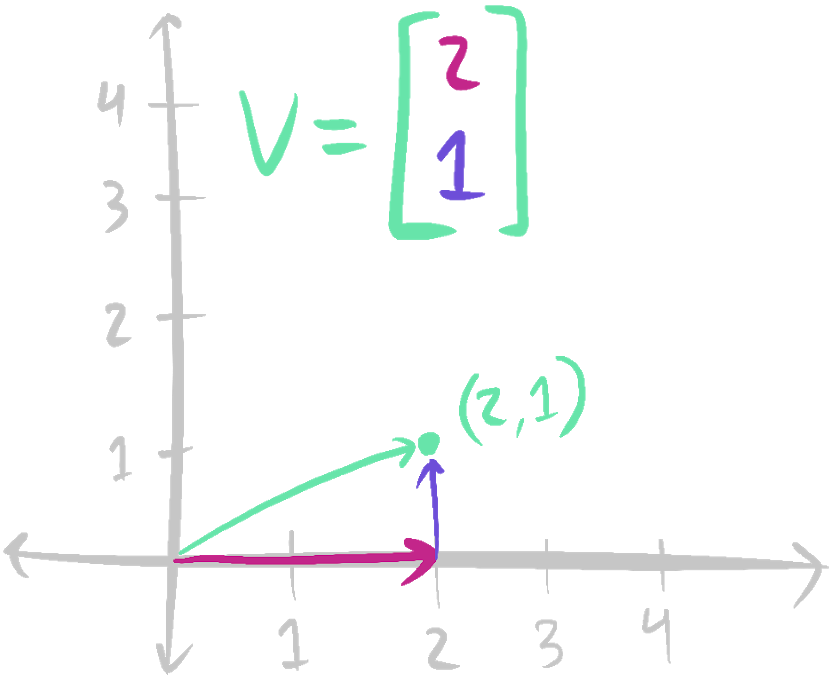
\includegraphics[width=2in]{figures/vector.png}
    \caption{Representing a 2-D vector graphically.}
    \label{vector}
\end{figure}

Matrices are the second fundamental component of linear algebra. These are \emph{two} dimensional arrays of numbers.
Each row and column of a matrix can be treated as their own vectors; they are called row vectors and column vectors respectively.
Additionally, vectors can be abstracted in terms of a matrix. For example, a 2-D vector could also be called a $2 \times 1$ matrix, as in Figure \ref{vectormatrix}.
\begin{figure}[hbt!]
    \centering
    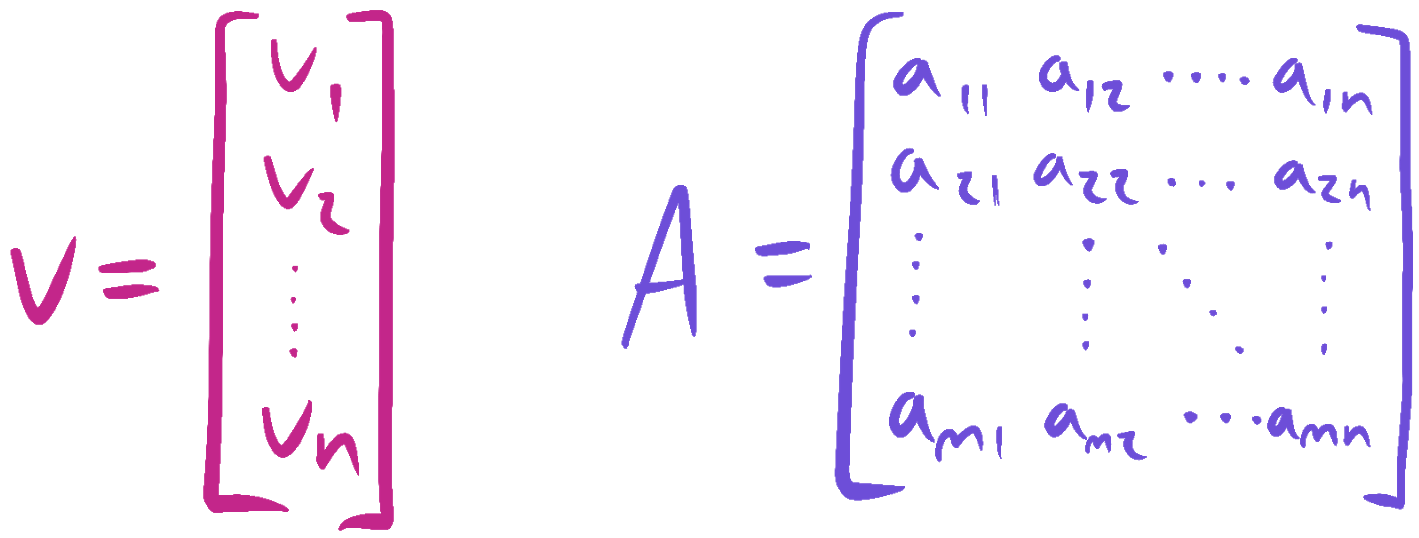
\includegraphics[width=3in]{figures/matrixvector.png}
    \caption{An example of a $n \times 1$ vector $\mathbf{v}$, and an $m \times n$ matrix $\textbf{A}$. }
    \label{vectormatrix}
\end{figure}
 We will later see why representing values with vectors and matrices is so useful and compact. Vectors and matrices come with their own sets of operations that can compress most of the mathematics we are dealing with.

\subsection{Matrix Multiplication}
The first operation we will discuss is called the \emph{dot product}. The dot product is a operation that ``multiplies" two vectors together to produce a scalar value. In order for this to be possible, both vectors must be the same size. For example, if there are two vectors $\textbf{v}$ and $\textbf{w}$, each with two elements, then the dot product would be $\textbf{v} \cdot \textbf{w} = v_1 w_1 + v_2 w_2$ (Figure \ref{dotproduct}).
\begin{figure}[hbt!]
    \centering
    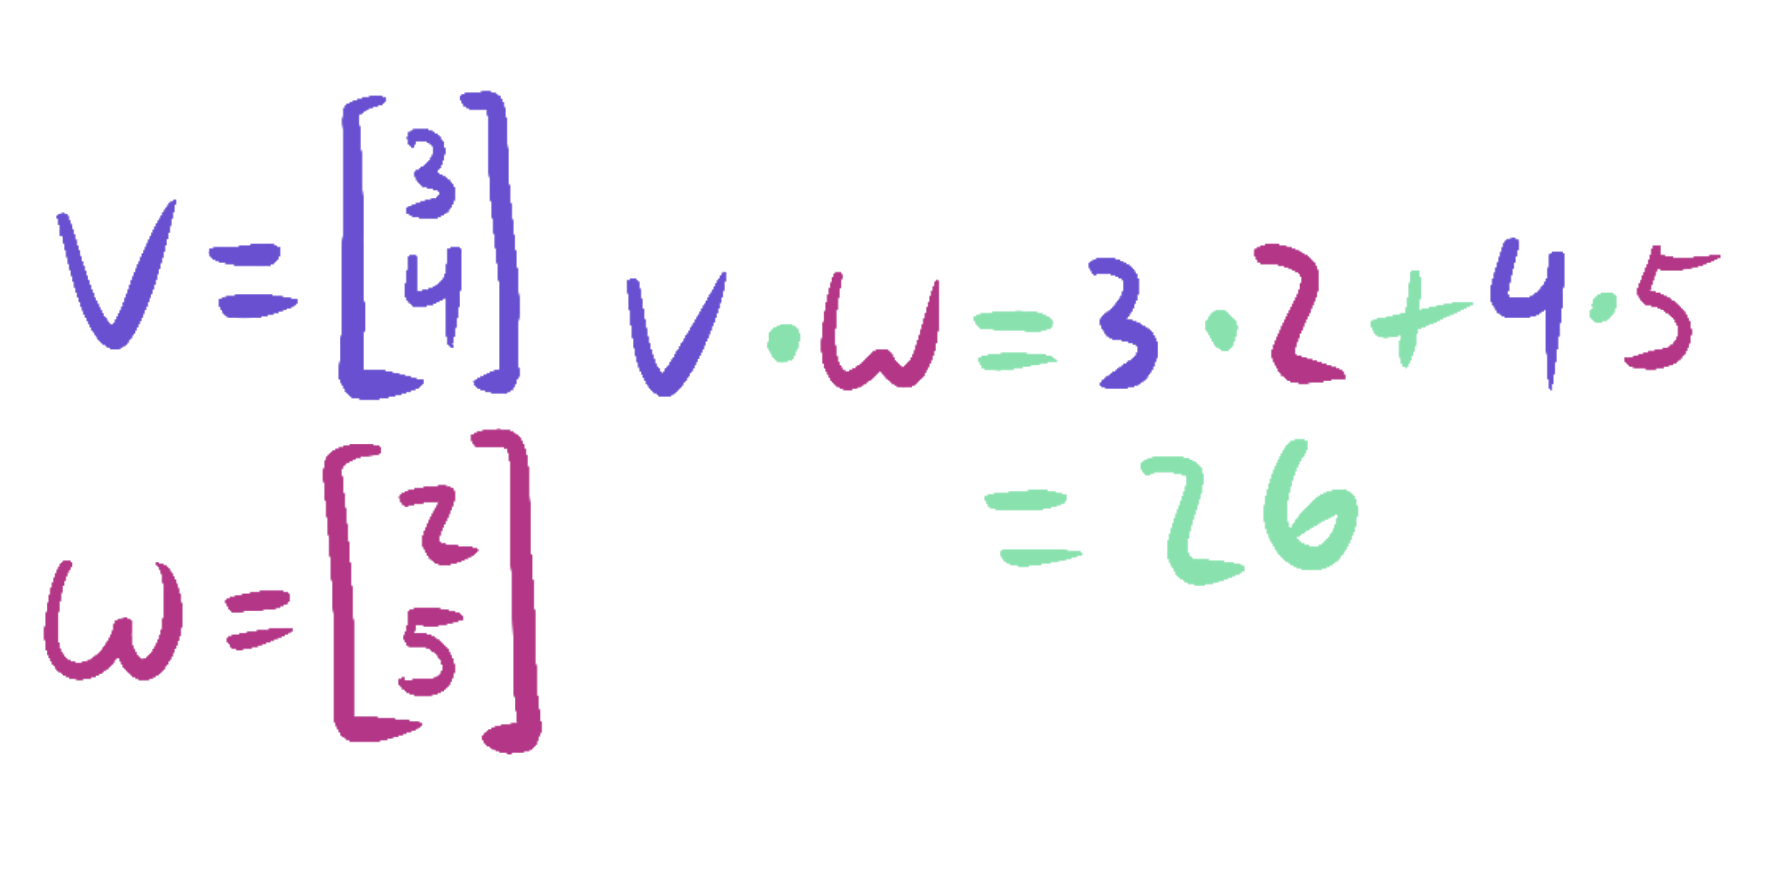
\includegraphics[width=3in]{figures/dotproduct.png}
    \caption{An example of the dot product of two 2-D vectors. }
    \label{dotproduct}
\end{figure}

With the dot product established, we can now address the second matrix operation, the \emph{matrix product}. The matrix product is a massive driving force behind Neural Networks. Like regular numbers or vectors, matrices can also be multiplied together, however, this process is much more complex. The matrix product considers every combination between the row vectors of the first matrix, and the column vectors of the second matrix, and produces a new matrix comprised of the dot products of those combinations. It can be quite a confusing concept; the example from Figure \ref{matmult} will make it more clear.
\begin{figure}[hbt!]
    \centering
    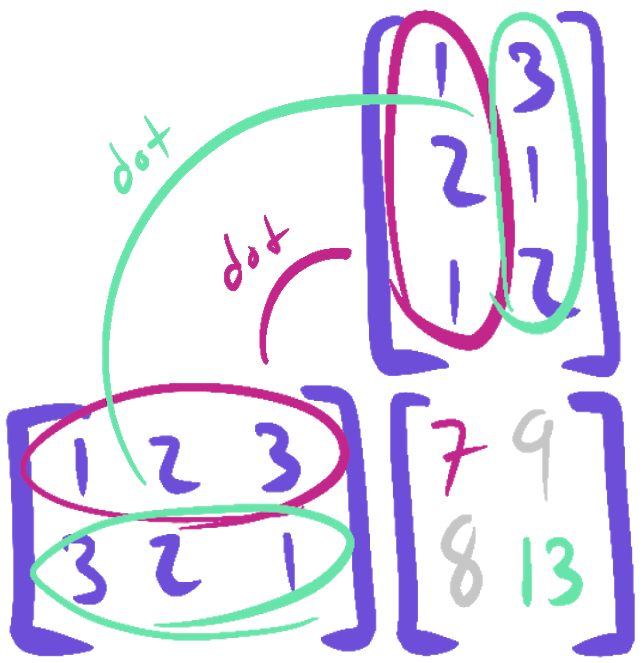
\includegraphics[width=1.75in]{figures/matmult.PNG}
    \caption{An example of a $2 \times 3$ matrix being multiplied with a $3 \times 2$ matrix to produce a $2 \times 2$ matrix.}
    \label{matmult}
\end{figure}

Similarly to how a vector is a special case of a matrix, the dot product is special case of matrix multiplication. A $1 \times n$ matrix, and an $n \times 1$ matrix are multiplied to produce a $1 \times 1$ matrix, which is the same as a scalar.

\subsection{Special Operations}
Lastly, I want to cover two additional types of matrix and vector operations that are not typically covered in an introductory linear algebra class, but are also important for understanding how a Neural Network functions. The first operations is called the \emph{Hadamard Product}. The Hadamard Product can best be described as an element wise multiplication between two matrices of the same size. This operation takes two matrices of the same dimension and outputs another matrix of the same dimension whose entries are the product of every corresponding entry of the two input matrices.
\begin{figure}[hbt!]
    \centering
    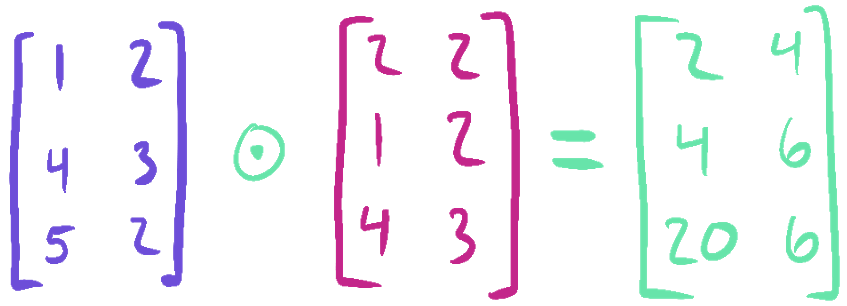
\includegraphics[width=2.5in]{figures/hadamard.PNG}
    \caption{An example of two $2 \times 3$ matrices being multiplied via the Hadamard Product.}
    \label{hadamard}
\end{figure}

The final operation we will cover is the \emph{outer product}. The outer product is an operation between two vectors, but instead of producing a scalar like the dot product, it produces a matrix. In other words, the outer product between an $m \times 1$ vector $\textbf{v}$, and a $1 \times n$ vector $\textbf{w}$, $\textbf{v} \otimes \textbf{w}$ will produce an $m \times n$ matrix. Like matrix multiplication, this can be confusing, and Figure \ref{outerproduct} will display the process more visually.
\begin{figure}[hbt!]
    \centering
    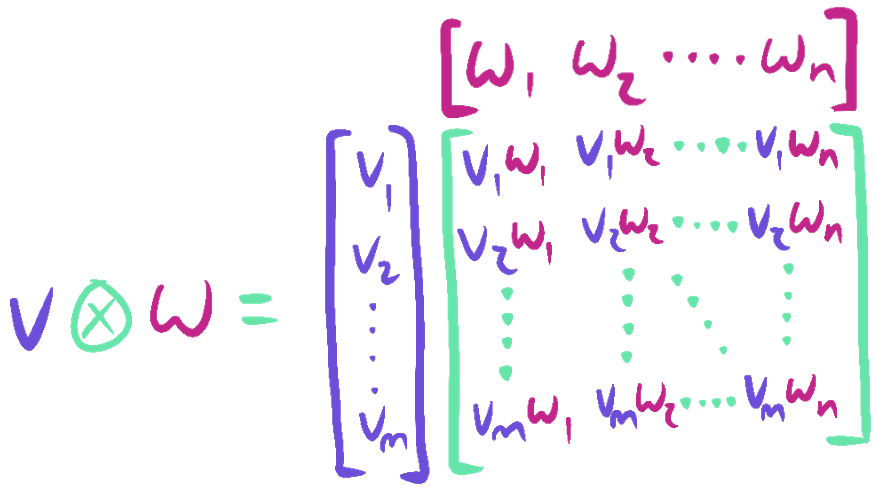
\includegraphics[width=2.5in]{figures/outerproduct.PNG}
    \caption{The outer product of an $m \times 1$ vector with an $n \times 1$ vector to produce and $m \times n$ matrix.}
    \label{outerproduct}
\end{figure}

Finally, all of the building blocks are in place, and we are ready to discuss the topics that motivate this project: Neural Networks, Hyperparameters, and Evolutionary Algorithms. The next section will outline the remainder of the report including the topics of each chapter, and their importance in the context of the project.

\section{Outline of Contents}
The purpose of this section is to briefly outline what is to come in the following chapters. This report also serves to explain the most important background concepts of the topic. Roughly half of the report is dedicated to background information of Neural Networks, hyperparameters,and genetic algorithms. The other half of the report is dedicated to the details of implementation for the project as well as the final results and reflections.

Chapter 2 will briefly cover the details of Neural Networks. Obviously, this is not an in depth explanation of every concept, since that would require a book's worth of information. Instead, Chapter 2 is meant to serve as an explanation to those already familiar, or lightly familiar with the topic already. Knowledge of calculus is assumed, and knowledge of linear algebra makes understanding easier. Topics covered in this chapter are artificial neurons, different network architectures, training and the back propagation algorithm, and a discussion of various activation functions, since this is an important piece of the project.

Chapter 3 introduces the problem, and thus the motivation for the project. It discusses what hyperparameters are and why they can make optimizing the performance of a Neural Network an very challenging problem. This is followed by a discussion of solutions in the form of evolutionary algorithms, hence the motivation of the project. There is also a brief discussion of how evolutionary algorithms work, and the particular type chosen for this project.

Chapter 4 discusses the details of implementation. We will walk through each class of the code in detail and discuss how every component of the Neural Network and Genetic Algorithm functions. This discussion is meant to elevate the understanding of someone who is not as comfortable or experienced with programming. The classes discussed are the Deep Neural Network architecture, the two classes that make up the genetic algorithm, and the class and script that run the evolution applied to the provided data.

Lastly, Chapter 5 will showcase the results and my reflections on those results. This is where the key pieces of project, and hence the final argument from the Abstract are solidified by the evidence of the results. Lastly, concluding remarks and a discussion of future steps for improving this work will be explored.

Appendices and references will be provided at the end. Please enjoy reading!

\chapter{A Crash Course in Neural Networks}
\label{cc}
Neural Networks are a hot subject. Thousands of books have been written over the past few decades, so attempting to teach Neural Networks from scratch would require its own book. Instead, the purpose of this chapter is to outline the fundamentals of Neural Networks, and the most important aspects about them. we will highlight the concepts that are relevant for the main research question. To start the discussion on Neural Networks, the best place to begin is with modern, real world applications that we encounter every day.

\section{Real World Applications}
Neural networks are a pretty common buzzword throughout tech company rhetoric and the media. But even if we look past the hype, we discover a huge set of possibilities. My favorite example of a problem Neural Networks can solve, is classifying hand written digits. Given a hand written input, the goal is to classify which digit between 0 and 9 the input represents. The research question seems fairly simple, but when we sit down and think about how to solve this problem in a traditional computer science fashion, the problem becomes very daunting. How can all possible cases be accounted for with such a large input? How can one programmer account for every possible rendition of what a ``2" or a ``4" is, since there are so many ways that they can be written?

As it turns out, Neural Networks solve this problem by allowing the engineer to circumvent hard coding every possible case. It is through this concept where the power of Neural Networks, and machine learning tactics like it, come to fruition! The process of a Neural Network ``learning" can even be thought of as one that automatically and heuristically accounts for every such case. It does this through data and approximation. The data is needed to provide enough examples for the architecture to learn which hand written digits correspond to which integers. The approximation occurs via the mathematics that powers the network. It is impossible to account for every possible input, and therefore every possible case. even with a computer. The typical problem suited for a Neural Network can have upwards of $10^{100}$ possible inputs. However, if enough data can be provided, the network can approximate a set of possible classifications for each hand written digit, regardless of the extremely large input space.

For example, imagine there is a calculus test that needs to be passed.
There is no reason for a student to study European history or sports medicine to do well on the test.
The best way for the student to prepare for the calculus test is to complete practice problems that have been on past calculus tests.
When problems similar to the practice problems appear on the test, the student will have learned the proper way to solve them, and is likely do well and score high.

\section{Neurons}
Let's first break apart what a Neural Network actually is. As the name suggests, a Neural Network is a collection of neurons, in a brain, connected together to process data \cite{mehlig2019artificial}.
In biology, neurons are comprised of three major parts: the input, which is made up of dendrites and synapses, the processing, which is made up of the cell body and nucleus, and the output which contains the axon and terminals.
See Figure \ref{bioneuron} for an illustration.
\begin{figure}[hbt!]
    \centering
    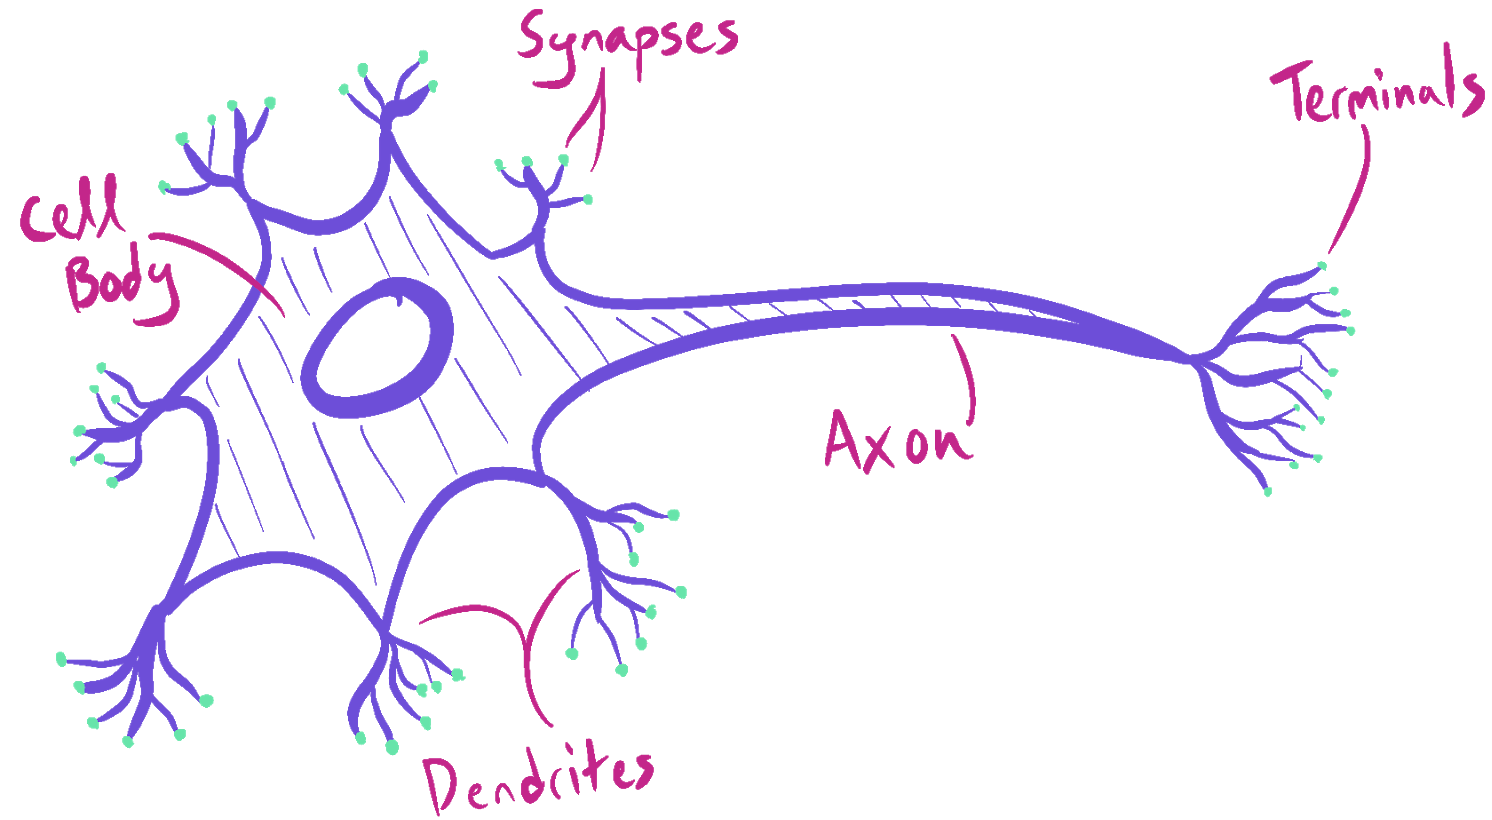
\includegraphics[width=3in]{figures/bioneuron.PNG}
    \caption{A schematic image of a neuron \cite{mehlig2019artificial}, showing the inputs, processing area, and outputs.}
    \label{bioneuron}
\end{figure}
The input part of a neuron receives information from all other neurons that feed into it. The main body of the neuron processes this information and activates, or ``fires'' its own signal. This signal is sent to all other neurons it feeds into via the axon and terminals. This is an extreme simplification, but it outlines the three important components that we try to replicate with an artificial neuron.

Compare this, to an artificial neuron, which adopts the same structure as a real neuron, but instead uses mathematics to handle processing tasks.
\begin{figure}[hbt!]
    \centering
    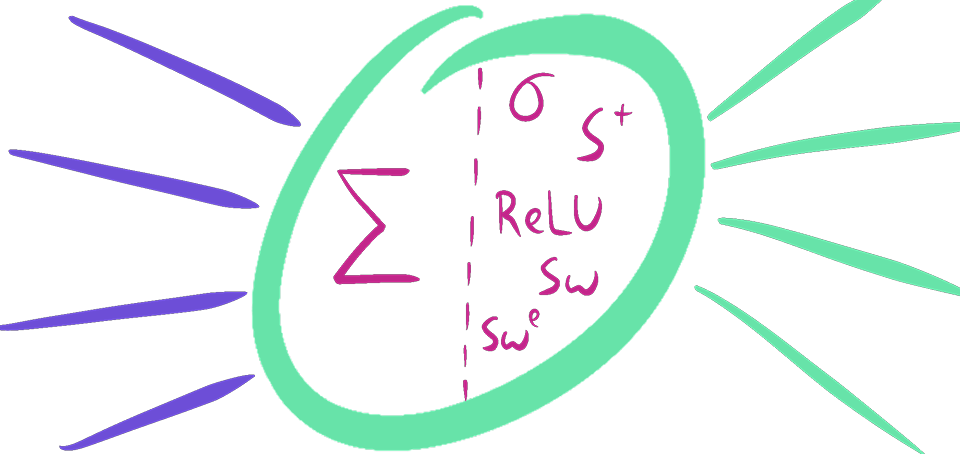
\includegraphics[width=3in]{figures/neuron.PNG}
    \caption{A model of an  artificial neuron, showing the inputs, processing area, and outputs.}
    \label{neuron}
\end{figure}
Artificial neurons are just complex functions that take a vector as an input and return a scalar value to each neuron it feeds into. As a result, an entire network of artificial neurons is really just an even more complex function that takes a vector as an input and produces a new vector as its output.

Each neuron contains two functions: the first one considers all the inputs from the nodes leading into it. This is called a basis function. The second function is called the activation function. It's purpose is to replicate the ``firing" of a biological neuron from an actual brain. There are several different types of activation functions, but there will be more details of activation function in Chapter \ref{section: activations}. In the next section, we will cover a few of the many different Neural Network architectures, especially the one used for this project.

\section{Architectures}
There are dozens of different types of Neural Network architectures. They all have their specific use cases, and many are complex expansions of older, more traditional models. The most important one for this project is the Multi-layer Perceptron (MLP), which most of our time will be dedicated to. However, we will also spend some time introducing more modern architectures at a high level, mainly for the sake of revealing the depth of the subject.

\subsection{Multi-Layer Perceptron (MLP)}
\label{mlp}
The MLP is a fundamental architecture that many of the more modern architectures today are built upon. It is a generalization of the simple perceptron, which was introduced as early as 1958 \cite{rosenblatt1958perceptron}. At that time, computers were not nearly as capable as they are today, so their viability as computational allies were extremely limited. Moreover, the mathematics that allow the Neural Network to actually ``learn" from the training data were not yet solidified. It was not until several decades later in the mid 1980s when the back propagation algorithm was first published, reawakening the viability of Neural Networks \cite{rumelhart1986learning}. Computers were significantly quicker, and used on a much larger scale. The usefulness of the perceptron, MLP, and deep MLP were thrust to the forefront of machine learning.

A Neural Network's artificial neurons are arranged into several layers.
All nodes between layers are fully connected, and the strength of these connections can be represented with a weight value $w$.
The number of layers a Neural Network has is called its ``depth".
For this project, a deep MLP architecture has been created with the capability of creating an MLP of any depth.

To illustrate with an example, consider an MLP with $n+2$ total layers.
The first layer is called the input layer, suppose it has dimension $p_0$.
The last layer is called the output layer; suppose it has dimension $p_{n+1}$.
The layers in between the input layer and the output layer are called hidden layers.
Thus there are a total of $n$ hidden layers each with dimension $p_i$ where $0 \leq i \leq n$.
Figure \ref{deepmlp} is an illustration of this example of an MLP with arbitrary depth.
\begin{figure}[hbt!]
    \centering
    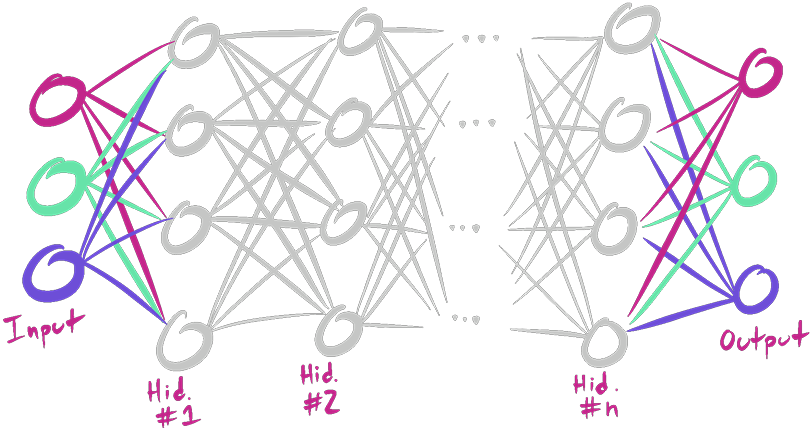
\includegraphics[width=3.5in]{figures/deepmlp.PNG}
    \caption{An MLP with input dimension 3, output dimension 3, and n hidden layers each with dimension 4.}
    \label{deepmlp}
\end{figure}
We will look at the details of what the connections between nodes on the network means and how the network actually learns in Chapter \ref{training}.
Next, we will very briefly go through a few more modern Neural Network architectures.

\subsection{Modern Architectures}
Now we will briefly look into two of the many more modern Artificial Neural Network architectures.
This first is called the Convolutional Neural Network (CNN), and the second is called the Recurrent Neural Network (RNN).
\subsubsection{Convolutional Neural Network (CNN)}
The CNN was first introduced in the late 1990s by Dr. LeCun and colleagues \cite{lecun1998gradient}.
This architecture has proven to significantly and consistently outperform the MLP, and as a result is the MLP's modern successor.
CNNs are used at the forefront of machine vision, image recognition, self driving cars, etc.
The reason for its success is due to the way it extracts features from the input data before feeding into a deep MLP.
We can see in Figure \ref{cnn} that this architecture has several pooling layers to reduce the input into a smaller set of features that are then used to train an MLP attached at the end of it.
\begin{figure}[hbt!]
    \centering
    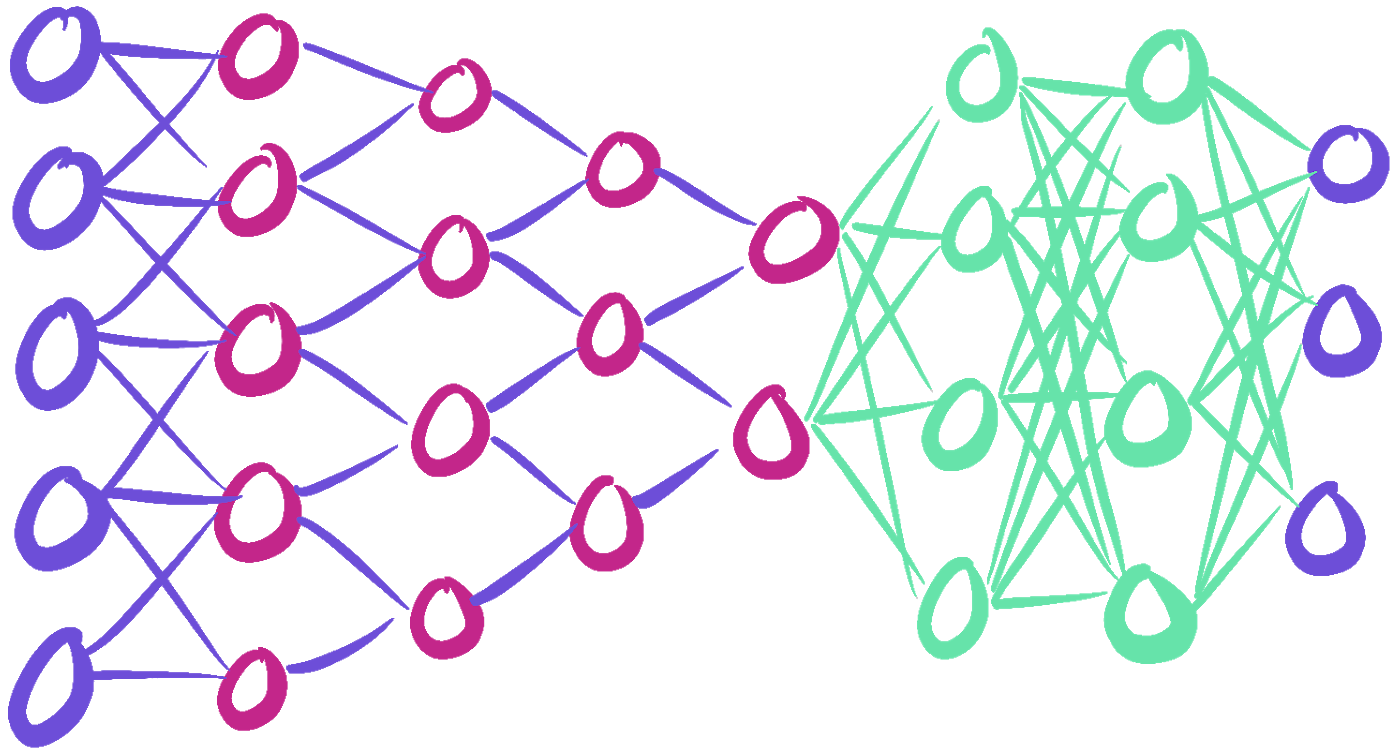
\includegraphics[width=3.5in]{figures/cnn.PNG}
    \caption{A basic diagram of a CNN.}
    \label{cnn}
\end{figure}

\subsubsection{Recurrent Neural Network (RNN)}
Similarly to the CNN, the RNN was also first introduced in the 1990s by Dr. Jeffery Elman \cite{elman1990finding}.
The RNN is very similar in structure to a regular MLP. The main difference is that the hidden layer nodes possess recurrent connections.
In other words, there are edges of the network that direct back into the node itself rather than just forwards or backwards. This allows the network to hold information through time. Essentially, recurrent connections give a node information about itself from the previous pass of training, while also taking inputs from the previous layer. Figure \ref{rnn} represents a basic diagram of a recurrent Neural Networks' topology.
\begin{figure}[hbt!]
    \centering
    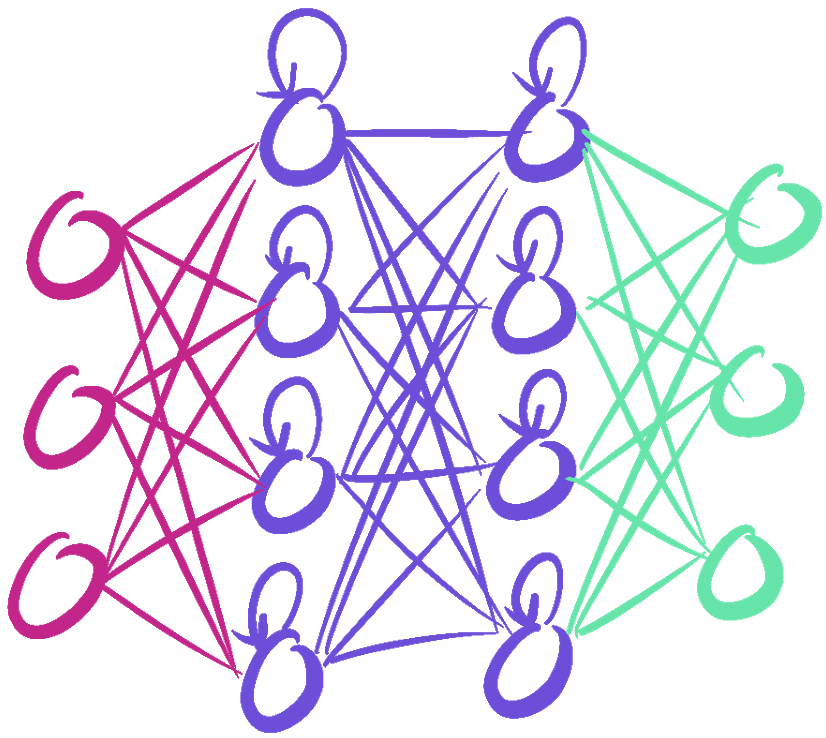
\includegraphics[width=2.5in]{figures/rnn.PNG}
    \caption{A basic diagram of a RNN.}
    \label{rnn}
\end{figure}

\section{Training}
\label{training}
Given what a Neural Network's structure actually looks like, and what we have covered about linear algebra and Neural Network basics thus far, we are ready to move on to the mathematical ``meat and potatoes" of what actually makes them work, and what it means for a Neural Network to ``Learn."
As mentioned before, we will be discussing in detail the mathematics behind the MLP architecture.
The entire process can be decomposed into two major parts: \emph{forward propagation} and \emph{backward propagation}(back propagation).

\subsection{Forward Propagation}
Recall, an MLP takes a vector as its input, where the dimension of that input vector corresponds with the total number of features being accounted for.
For example, if the goal is to predict the price of gas in your area, then the time of year, price of oil, and average distance from other gas stations could all be used as features to make this prediction.

To illustrate this mathematically, assume an MLP like the one from Chapter \ref{mlp}.
Let $\textbf{a}_0$ be the input vector with dimension $p_0$ for one particular training example.
Furthermore, let $\textbf{a}_{n+1}$ be the output vector of dimension $\textbf{p}_{n+1}$ after forward propagation. We need to ``feed" this information forwards through the network in a way that produces a meaningful result as the output. In the case of our example, we want some value that represents the price of gas per gallon given the three aforementioned input features.

Recall Figure \ref{neuron}. There are two functions applied within each neuron. The first function, called the linear basis function, sums the input from all nodes in the previous layer multiplied by the connection weight $w$. Second, the neuron outputs some ``activation" based on the linear basis function. This activation is the output that serves as the input to the next layer until the final layer is reached.

Now consider the first hidden layer, $\textbf{a}_1$, with dimension $p_1$.
Since each of the connections between every node in $\textbf{a}_0$ and every node in $\textbf{a}_1$ have a corresponding weight, we can represent all of them at once with a weights matrix $\textbf{W}_0$, where each weight $w_{i,j}$ indicates the specific weight of a connection from node $i \in \textbf{a}_0$ to node $j \in \textbf{a}_1$. Also note that $0 \leq i \leq p_0$ and $0 \leq j \leq p_1$.
There is also a bias value that must be added separately to each of the nodes in the next layer. This can be done with a vector $\textbf{b}_0$. This is essentially the same as having a zeroth column as the bias in the weights matrix \cite{krose1996introduction}.

So, beginning the forward propagation, let $\textbf{s}_1$ be the resulting vector from applying the linear basis function to each node from $\textbf{a}_0$, which can be completed in one step as a matrix multiplication. So, we see that the linear basis function of our input vector is simply:
$$\textbf{s}_1 = \textbf{W}_0 \textbf{a}_0 + \textbf{b}_0$$
Now, we apply some arbitrary activation function $f(x)$ to the vector $\textbf{s}_1$ to get the activation for our next layer: $\textbf{a}_1$.
It's important to note that a scalar function can take in vector input and produce a vector as its output by applying the function to each individual entry of the vector.
This allows for the forward propagation of an entire input to be compacted down to one simple formula \cite{youtube_2017}:
$$\textbf{a}_1 = f(\textbf{W}_0 \textbf{a}_0 + \textbf{b}_0)$$
Now we have successfully moved from the input layer to the first hidden layer, and the next step is to continue forward. We see that given $\textbf{W}_0, ... ,\textbf{W}_{n+1}$ and $\textbf{b}_0, ... ,\textbf{b}_{n+1}$ we can represent forward propagation recursively as follows:
$$\textbf{a}_j = f(\textbf{W}_{j-1} \textbf{a}_{j-1} + \textbf{b}_{j-1})$$
where $1 \leq j \leq n+1$.

\subsection{Error}
Once the output activation has been reached the output can be compared with target values that represent the expected output of the network. The target values allow for the calculation of error, which is important for two main reasons. First, error is a metric for measuring the performance of the network given the set of weights it has. Initially, the network's performance is likely to be very poor because it has not yet ``learned" from the data. Over time and with enough training examples, the network's weights will eventually be adjusted to minimize this error. This happens during the back propagation phase which is the second main reason error is important. Calculating error is extremely simple, we just subtract the target values, which we will call $\textbf{y}$, from the output values. Let's call this error vector $\boldsymbol{\epsilon}_0$.
Therefore we have:
$$\boldsymbol{\epsilon}_0 = \textbf{a}_{n+1} - \textbf{y}$$
The overall error for the entire training set is the sum of the squares of every error value. Taking this sum, we get a value that we will call $\hat{E}$ which represents the overall performance of the network across all training examples. So, the squared error is
$$\hat{E} = \sum_i \boldsymbol{\epsilon}_{0i} \cdot \boldsymbol{\epsilon}_{0i}$$
where $i \in I$ is the index set of all the training examples.

\subsection{Back Propagation}
The final phase of training is to adjust the weights matrices in order to minimize the squared error. The best way to do this is by calculating the small changes, or partial derivatives, between every node from one layer to the next. This is not as intimidating as it seems, though, because the partial derivatives can also be expressed in the vector notation, and the relationship between one layer and the last can be established recursively! The error $\boldsymbol{\epsilon}_0$ represents the error from $\textbf{a}_{n+1}$. So, we can essentially calculate an ``error value" for each layer in the network. Let the vector containing the partial derivatives for $\boldsymbol{\epsilon}_0$ be $\textbf{d}$. The partial derivatives are the Hadamard product of the error values with the \emph{derivative} of the activation function on the previous layer:
$$\textbf{d}_0 = \boldsymbol{\epsilon}_0 \odot f'(\textbf{a}_n)$$
Hence, the error value for $\textbf{a}_n$ can be calculated with $\textbf{W}_n$ multiplied by the previous composition
$$\boldsymbol{\epsilon}_1 = \textbf{W}_n \textbf{d}_0$$
$$\boldsymbol{\epsilon}_1 = \textbf{W}_n (\boldsymbol{\epsilon}_0 \odot f'(\textbf{a}_n))$$
Again, we can now expand this recursive relationship until we reach the input layer.
$$\boldsymbol{\epsilon}_j = \textbf{W}_{n+1-j} (\boldsymbol{\epsilon}_{j-1} \odot f'(\textbf{a}_{n+1-j}))$$
again where $1 \leq j \leq n+1$.

Lastly, the partial derivatives matrix, which is used for adjusting the weights, can be constructed by taking the outer product of the partial derivatives vector $\textbf{d}_0$ with the previous activation vector $\textbf{a}_n$. Since the dimensionality of $\vec{d}$ will be $p_{n+1}$, and the dimensionality of $\textbf{a}_n$ is $p_n$, their outer product produces an $p_{n+1} \times p_n$ matrix representing the partial derivatives of $\textbf{W}_n$ for one training example. We will call this matrix $\textbf{C}_n$ and the formula for one particular training example is
$$\textbf{C}_0 = \textbf{d}_0 \otimes \textbf{a}_n$$
Recursively, we get
$$\textbf{C}_j = \textbf{d}_j \otimes \textbf{a}_{n-j}$$
with $0 \leq j \leq n$.
This process is repeated for every training example, and after every training example has been assessed a final matrix of the accumulated values is used to update the weights all at once. Let $\mathscr{C}_j$, hence we have
$$\mathscr{C}_j = \sum_i \textbf{C}_i$$
again where $i \in I$ represents the index set of all training examples.
The bias vector also needs to be updated, but since the ``activation" value for the biases is always one, its the same as taking the sum across all training examples of the partial derivatives vector.
$$\boldsymbol{\beta} = \sum_i \textbf{d}_j$$

A small proportion of the changes in the weights and biases are then subtracted from the network's actual weights and biases so that there will be less error when training on the next pass of the data. These passes are known as \emph{epochs}, and the small proportion value for making the adjustment is called the \emph{learning rate}. A learning rate that is too high may not be able to converge to a minimum on the error function's surface.

\section{Activation Functions}
\label{section: activations}
In the previous section, we covered the details of what it means when a Neural Network is training and learning. In these explanations, however, we used $f(x)$ to represent an arbitrary activation function for the neurons. In this section, we will cover a series of well known, and actively used activation functions, and discuss why some are used more predominantly than others.
\subsection{Sigmoid}
The first activation function the classic and original activation function called the \emph{Sigmoid} Activation Function. The Sigmoid function is defined as
$$\sigma(x) := \frac{1}{1+e^{-x}}$$
and is graphed in Figure \ref{sigmoid}.
\begin{figure}[hbt!]
    \centering
    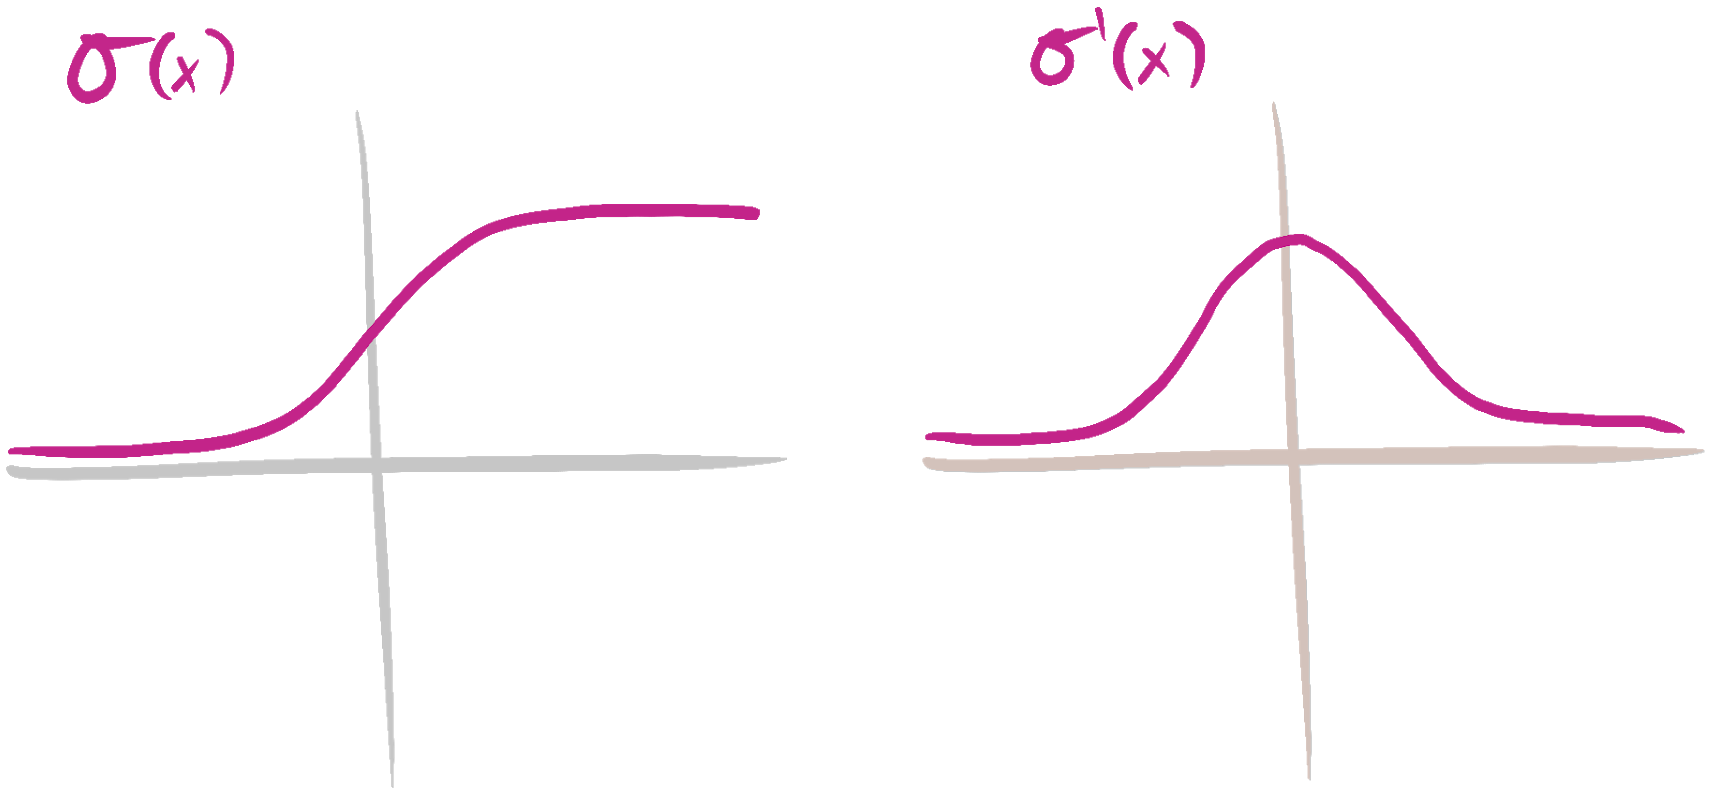
\includegraphics[width=3.5in]{figures/sigmoid.PNG}
    \caption{Sigmoid activation function (right) and its derivative (left).}
    \label{sigmoid}
\end{figure}
The purpose of this function is to take the value of each node after applying the linear basis function and ``squish" that value into a new value between 0 and 1, which represents the new activation of the next layer. This function is continuous everywhere and has the derivative
$$\sigma'(x) = \sigma(x)(1 - \sigma(x))$$

However, for as reliable and consistent as this function is in Neural Networks, it also has its own problems. The derivative for very large, or very negative inputs will be very close to 0 which can cause the partial derivative matrices to converge to zero, thus not significantly updating the weights and biases ever. This is known as the disappearing gradient problem. However, since its conception there have been dozens of new activation functions introduced into the literature that have taken the place of sigmoid because they are faster, better performing, and are actively being used today.

\subsection{ReLU}
The main successor to the Sigmoid function is the \emph{Rectified Linear Unit}. This is a much simpler activation function defined as
$$\text{ReLU}(x) := \text{max}(0,x)$$
Unlike the sigmoid activation function, the activation of a neuron is unbounded in the positive direction, and if the result from the linear basis function is negative, then there is no firing of the neuron at all. The function graph can be seen in Figure \ref{relu}.
\begin{figure}[hbt!]
    \centering
    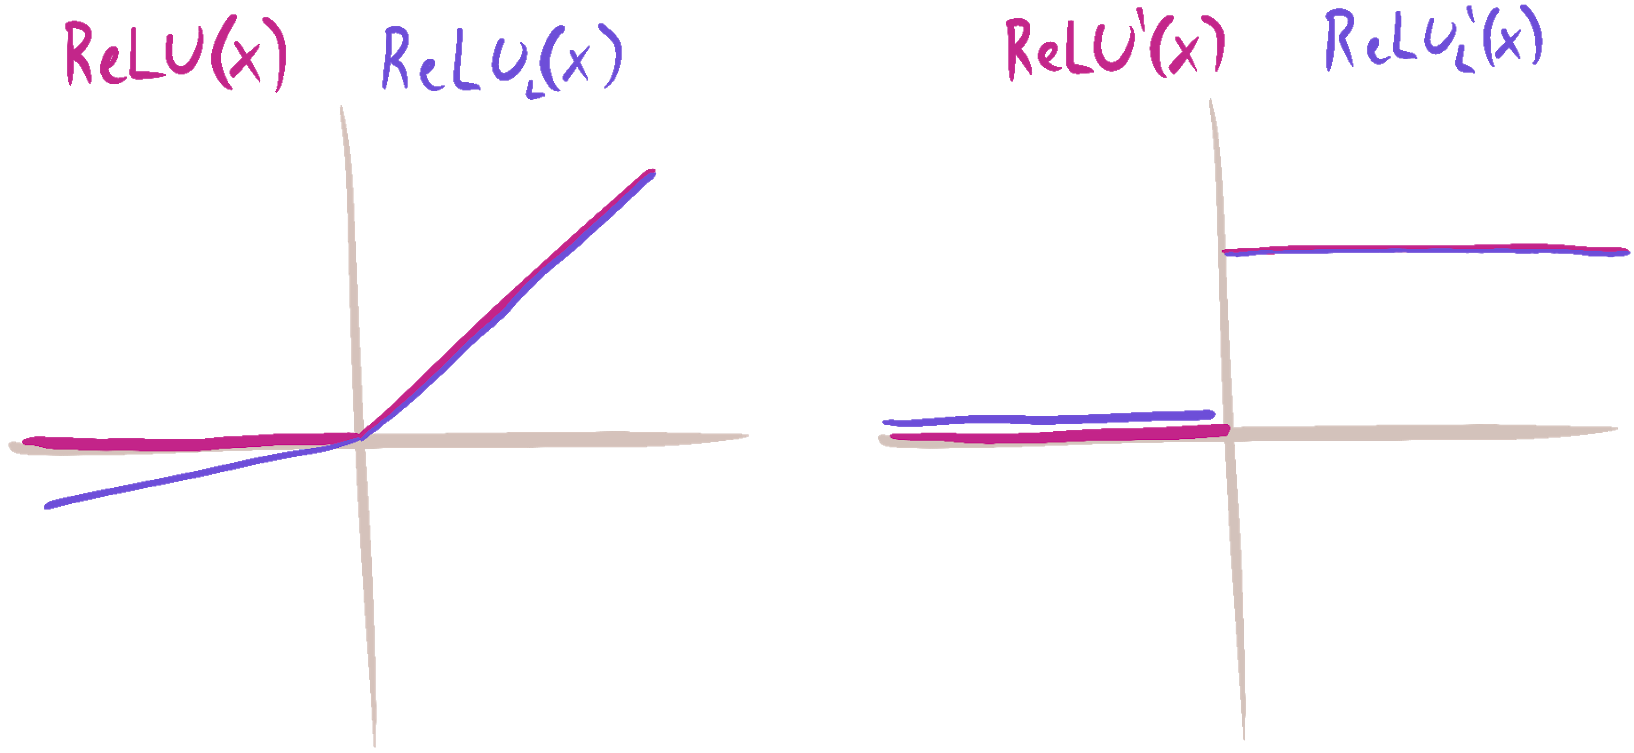
\includegraphics[width=3.5in]{figures/relu.PNG}
    \caption{ReLU activation functions (right) and their derivatives (left).}
    \label{relu}
\end{figure}
This activation function helped spark what some call the end of the second A.I. winter. I think its simplicity and performance also make Neural Networks more accessible as a whole, since the derivative can be represented as
$$\text{ReLU}'(x) :=
\begin{cases} 
0 & x < 0 \\
1 & x \geq 0
\end{cases}$$

In addition to the standard ReLU function, there is a variant activation function called the Leaky ReLU function, also in Figure \ref{relu}, defined as
$$\text{ReLU}_L(x) :=
\begin{cases} 
ax & x < 0 \\
x & x \geq 0
\end{cases}$$
where most often, $0 \leq a \leq 1$.
This function has derivative
$$\text{ReLU}_L'(x) :=
\begin{cases} 
a & x < 0 \\
1 & x \geq 0
\end{cases}$$
The key difference is that that there is an activation for values that are less than zero, just at a significantly reduced proportion. There is evidence to suggest that this is a slightly better performing activation than the original ReLU, but this claim is mostly observational \cite{xu2015empirical}.

\subsection{Swish}
The last category of activation functions are very similar to rectified linear units, but they are continuous functions instead of piece-wise functions. The first represents an ``interpolation" of ReLU, and it is called the \emph{Softplus} Activation function.
$$\text{S}^+(x) := \ln(1 + e^x)$$
Interestingly, this function is the anti-derivative of the Sigmoid function!
So, it is not too difficult to understand because it is part of the Sigmoid family.
Figure \ref{softplus} shows the graph of this function.
\begin{figure}[hbt!]
    \centering
    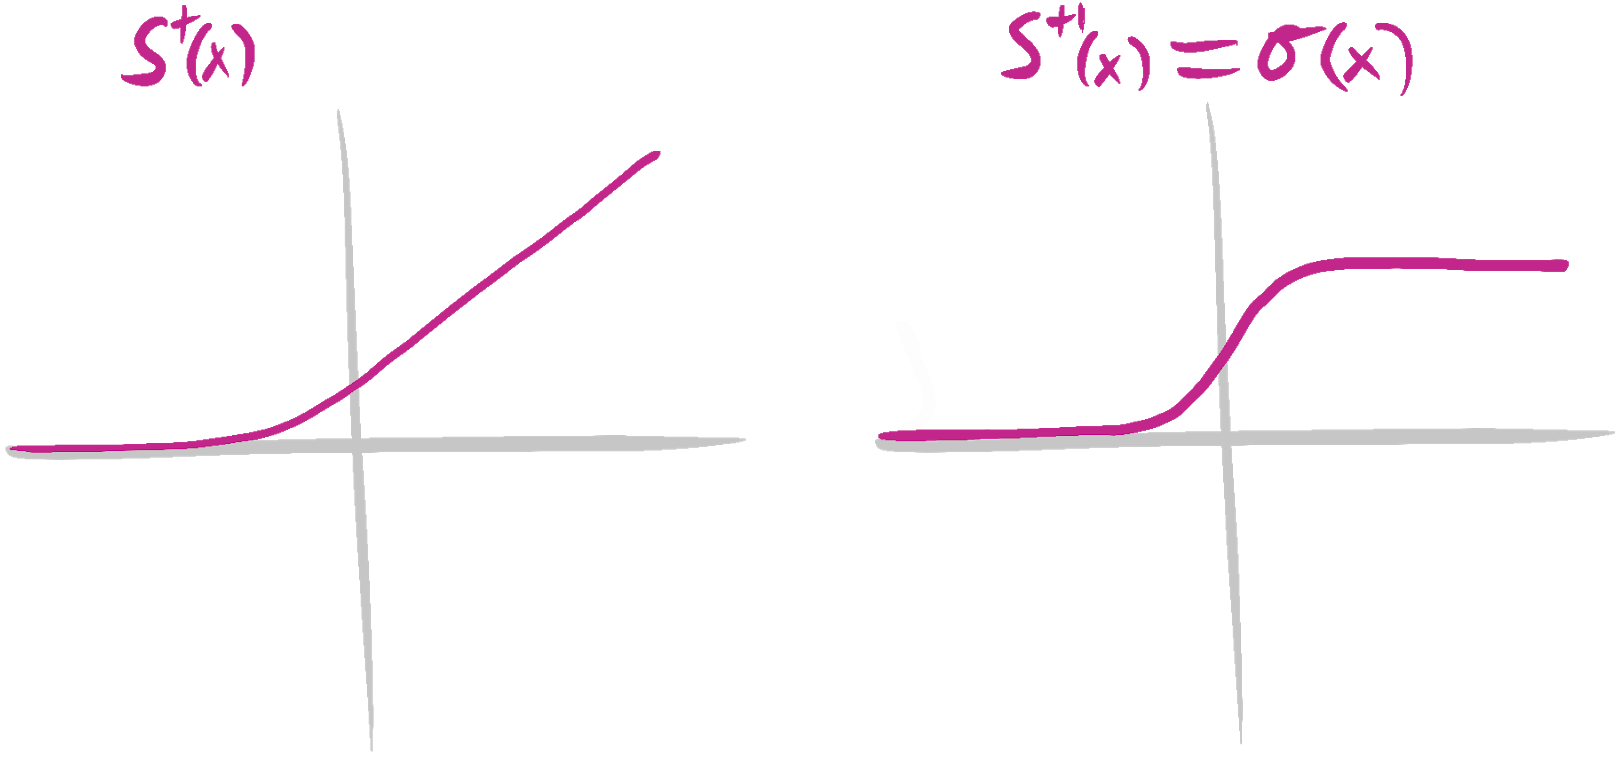
\includegraphics[width=3.5in]{figures/softplus.PNG}
    \caption{Softplus activation function (right) and its derivative, the sigmoid function (left).}
    \label{softplus}
\end{figure}

The next two functions are very interesting, because they are both similar to one another, but much better continuous approximations of the ReLU functions. The first one is called the \emph{Swish} Activation function \cite{ramachandran2017searching}. The formula for the swish activation function is given partially in terms of the Sigmoid activation function as
$$\text{Sw}(x) := x \sigma(\beta x)$$
and can be seen in Figure \ref{swish}.
\begin{figure}[hbt!]
    \centering
    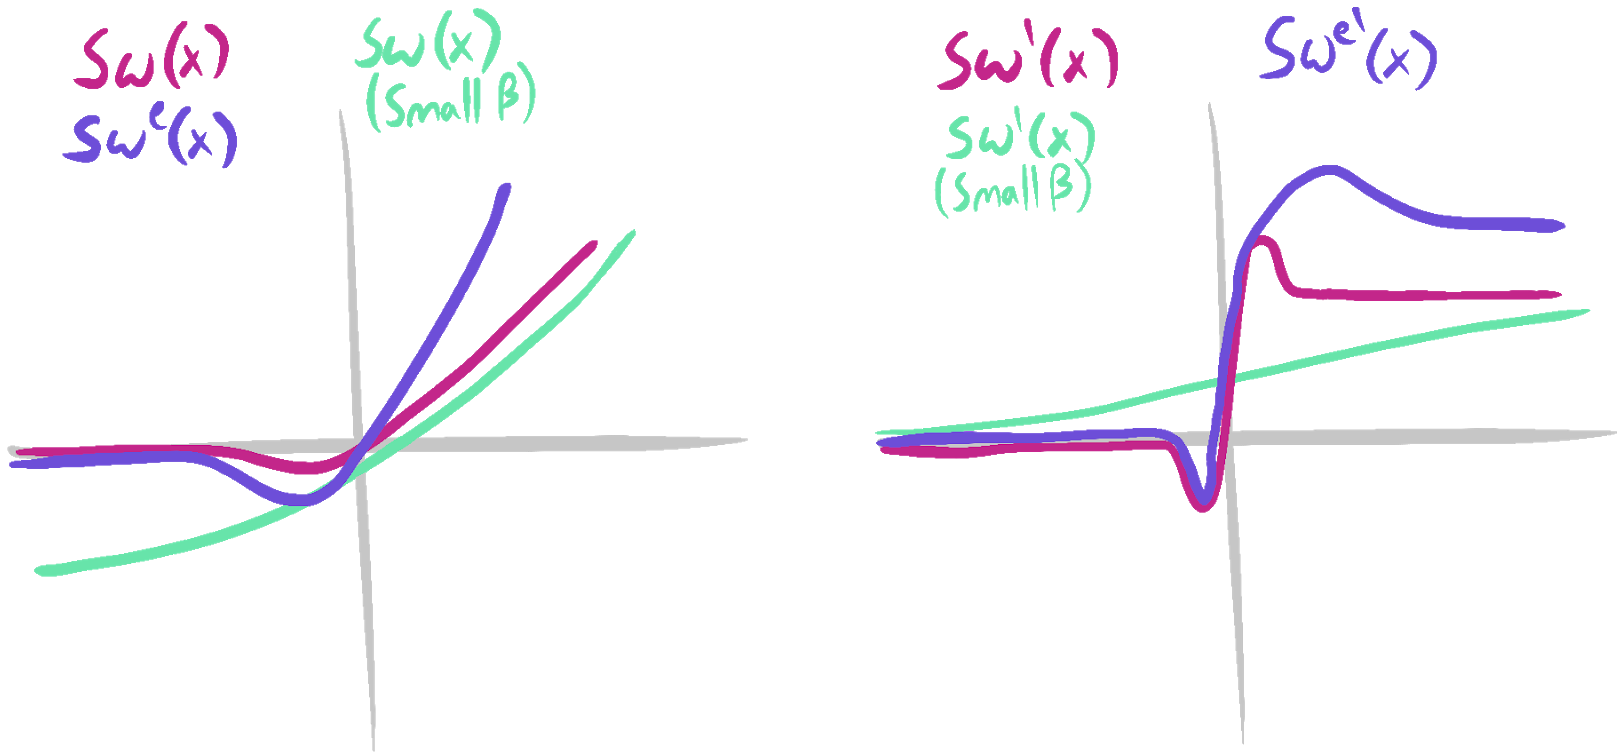
\includegraphics[width=3.5in]{figures/swish.PNG}
    \caption{Swish and E-swish activation functions (right) and their derivatives (left).}
    \label{swish}
\end{figure}
The derivative is slightly more complicated than sigmoid, though. Because of the chain rule we get the derivative as 
$$\text{Sw}'(x) = \sigma(\beta x) + \beta \text{Sw}(x) (1 - \sigma(\beta x))$$
In their paper, this function possesses a parameter $\beta$ that essentially controls the ``smoothness" of the function. What makes the swish activation function really interesting is that as $\beta \rightarrow \infty$, the function $\text{Sw} \rightarrow \text{ReLU}$.

Finally, we will briefly cover another variant of Swish called the \emph{E-swish} Activation Function \cite{alcaide2018swish}. The function formula is
$$\text{Sw}_e(x) := \beta x \sigma(x)$$
and it is also represented graphically in Figure \ref{swish}.
This function is very similar to the regular swish function, but it adds an extra parameter on the outside, $\beta$, which is claimed to have a slightly better result than swish; typically $1 \leq \beta \leq 2$. The derivative is slightly different from that of the Swish function:
$$\text{Sw}_e'(x) = \beta \sigma(x) + \text{Sw}_e(x) (1 - \sigma(x))$$

Having a variety of activation functions to choose from is very useful, because some functions can outperform others given a specific problem.
Therefore having more options allows for more opportunity to optimize the model.
This concludes the discussion of different activation functions and their importance. Next we will discuss how in why picking the right combination of attributes for a specific neural network can be such a complex task.

\chapter{Hyperparameters and the Problems They Cause}
Many machine learning algorithms require their own set of parameters to function, and Neural Networks are certainly no exception! As we will see in this chapter, understanding how to pick the right parameters for these models can create a lot of unforeseen problems.

\section{Introduction to Hyperparameters}
As we have explored during Chapter \ref{cc}, there are many ways to construct a Neural Network. It can have arbitrary depth, each hidden layer can have an arbitrary number of nodes, the activation function can vary, etc.
Every Neural Network has a set of parameters governing its structure that must be decided upon when creating the actual network. These are called \emph{hyperparameters}. Hyperparameters are the components of the Neural Network that are decided upon by the creators, given the context of the problem they are trying to solve. These decisions could be based on prior experience, trial and error, or even arbitrarily. And while there are standard conventions that have become accepted from the thousands of trial and errors over the decades, it is still the case that these conventions are just general guidelines. As it turns out, finding the optimal set of hyperparameters to use on a specific network for a specific problem is an extremely difficult task.

To begin addressing this, let's first think of a way to represent hyperparameters. There is a paper by Matthias Feurer and colleagues that explains the idea of hyperparameters as part of a \emph{hyperparameter space}.
\begin{figure}[hbt!]
    \centering
    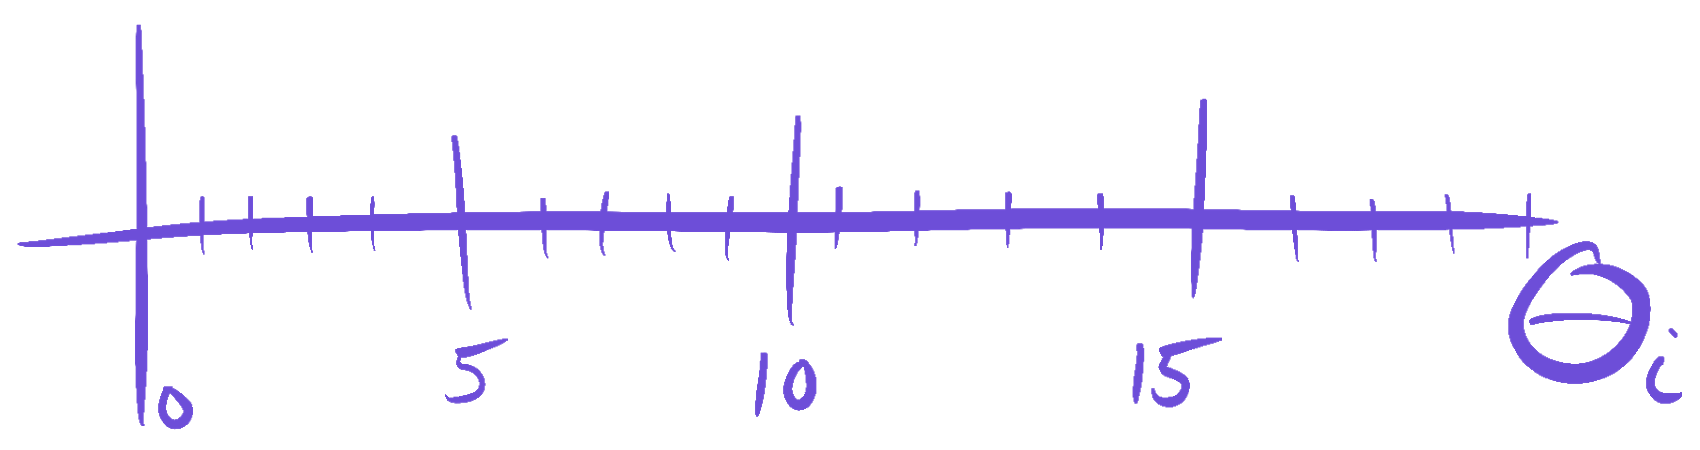
\includegraphics[width=3in]{figures/plot-1d.PNG}
    \caption{Any specific hyperparameter domain.}
    \label{plot-1d}
\end{figure}
This is a fairly mathematical way to conceptualize hyperparameters, but it illustrates why trying to search for the best hyperparameters can be so difficult. ``Let $\theta_1, ...., \theta_n$ denote the hyperparameters of a machine learning algorithm, and let $\Theta_1,..., \Theta_n$ denote their respective domains. The algorithm's hyperparameter space is then defined as $\bf{\Theta} = \Theta_1 \times \cdot \cdot \cdot \times \Theta_n$" \cite{feurer2015initializing}. Figures \ref{plot-1d}, \ref{plot-2d}, an \ref{plot-3d} all illustrate an example of what a hyperparameter space would be in one, two, and three dimensions respectively.
\begin{figure}[hbt!]
    \centering
    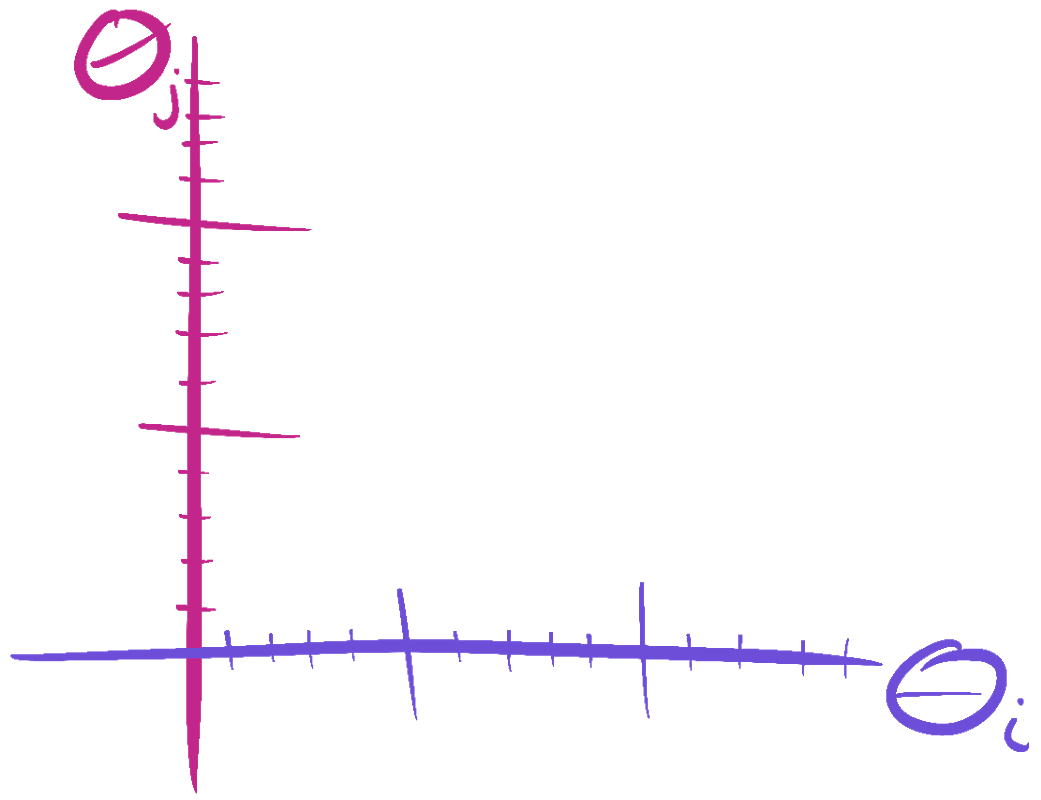
\includegraphics[width=2.5in]{figures/plot-2d.PNG}
    \caption{A two dimensional hyperparameter space.}
    \label{plot-2d}
\end{figure}

\begin{figure}[hbt!]
    \centering
    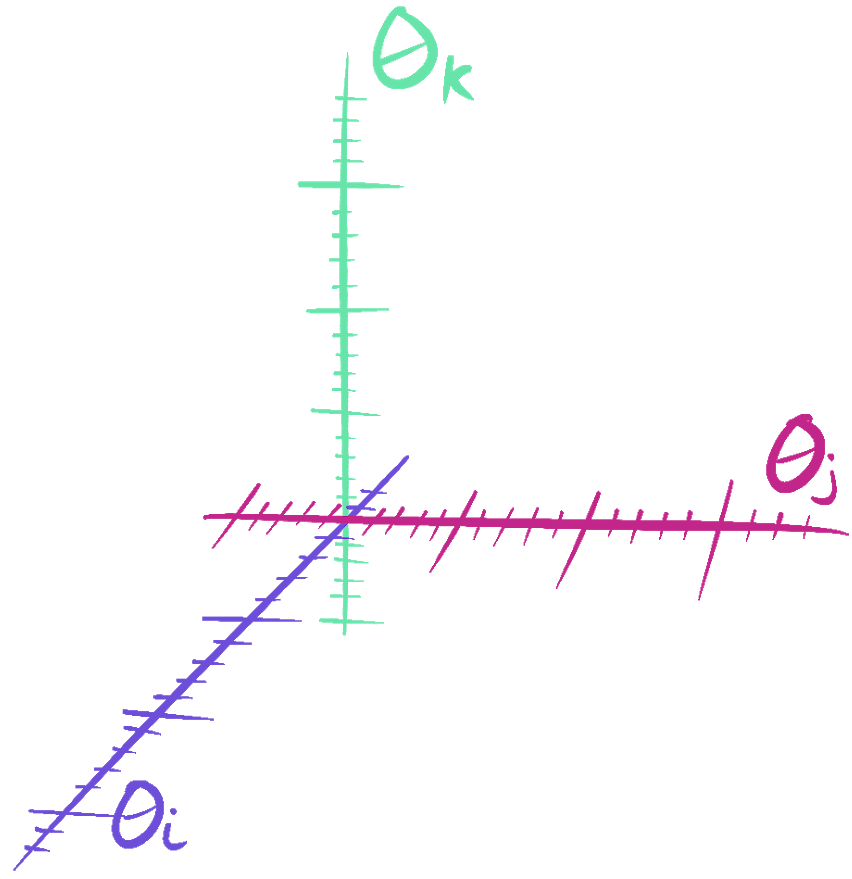
\includegraphics[width=2.5in]{figures/plot-3d.PNG}
    \caption{A three dimensional hyperparameter space.}
    \label{plot-3d}
\end{figure}

From these examples, it is easier to understand what is meant by ``high dimensional" hyperparameter spaces.
Moreover, by thinking about a hyperparameter in terms of a position in Euclidean Space, it is much easier to think about what it means to pick a set of hyperparameters as a vector being represented in that space.
In other words, the number of possible hyperparameters is equivalent to $2^{|\Theta_1| \times \cdot\cdot\cdot \times |\Theta_n|}$. Hence, there exists at least one point in this space such that it produces optimal results for our Neural Network. All we need to do is find such a point.

\section{NP Problems}
The problem with finding such a set of hyperparameters is it can be extremely computationally expensive to search for that magic point in the hyperparameter space. Notice that a brute force search for these hyperparameters would result in an algorithm with running time $O(2^n)$. Essentially, as the number of different hyperparameters increases, the more likely it will be impossible for a computer to finish the search before the heat death of the universe. This is what's known as an NP problem.

The world is full of NP problems. These are problems that can only be solved in non-deterministic polynomial time. One of the major issues with this kind of problem is that given a certain, not necessarily large, input size, the computation time becomes unpractical very quickly. An example of this is the ``Traveling Salesperson" problem. The idea is, given n cities, the traveling salesperson ``will conduct a journey in which each of his target cities is visited exactly once before he returns home" \cite{dasgupta2008algorithms}. By analyzing the time complexity of such a problem, we see that ``there are at most $2^n$ sub-problems, and each one takes linear time to solve. The total running time is therefore $O(n^22^n)$" \cite{dasgupta2008algorithms}. So, as the number of cities n increases, the total calculation time diverges to unfathomable amounts.

\section{Shortcuts for solving These Problems}
While the brute force approach to solving these problems is guaranteed to produce the optimal solution, there are alternative approaches that perform well and don't involve testing every single possibility. These methods can be used to approximate non-deterministic polynomial problems with polynomial solutions, and this section will be dedicated to explaining a few of those techniques.

\subsection{Manual, Random, and Grid Search}
Currently, there are three predominant ways of searching for hyperparameters, all of which have benefits and limitations. The three most widely used methods for hyperparameter selection in deep learning are (1) manual search, (2) grid search, and (3) random search \cite{young2015optimizing, bergstra2012random}. Manual search is the aforementioned ``Trial and Error" approach, which is the least time consuming, but also the least likely to be optimal or near optimal. Grid search is essentially the same as a brute force search, where an algorithm scans across the hyperparameter space fixing $n-1$ parameters and searching one parameter at a time. It is not actually a polynomial solution to this problem. Grid search wastes resources exploring what could be unimportant dimensions of the hyperparameter space while holding all other values constant \cite{young2015optimizing}. Random search can eliminate the problem of wasting resources in unnecessary dimensions of the hyperparameter space, but at, again, a loss in optimality.

\subsection{Heuristic Search and Genetic Algorithms}
In order to tackle these types of problems, people needed to think in an entirely new way. Inspired by biology, heuristics, and holism, Genetic Algorithms (GAs) are a biologically inspired heuristic search or optimization algorithm. And while heuristic solutions are usually not optimal, they are near optimal for a negligible proportion of the computational effort.

A GA functions on the same principles that embody Charles Darwin's theory of evolution via natural selection. A population of computational organism all have a set of DNA that encodes for one specific solution to the problem. There is some type of objective function that the performance of each organism can be evaluated on, and this performance measurement represents the fitness of that organism. Like biological natural selection, the artificial organisms with higher fitness values are more likely to reproduce, in which some of the DNA from each of the parents are sampled and combined to make offspring organisms with a new encoded solution based on the two parents' DNA. Additionally, the reproduction process can also have mutations. These mutations can introduce chances to increase fitness over several generations.

Dr. John Holland metaphorically explains why GAs ability to search in high dimensional space is superior to brute force. ``As the number of dimensions of the problem space increases, the countryside may contain tunnels, bridges and even more convoluted topological features. Finding the right hill or even determining which way is up becomes increasingly difficult...Genetic algorithms cast a net over this landscape. The multitude of strings in an evolving population samples it in many regions simultaneously" \cite{10.2307/24939139}. Therefore, using an evolutionary algorithms approach to optimize the hyperparameters of a Neural Network seems like a viable approach to solving the problem.

The genetic algorithm for this project will be based on the conventions of Dr. Goldberg's Simple Genetic Algorithm (SGA). The reproduction phase implements methods from Goldberg's SGA such as elitism, hermaphroditic sexual reproduction based on the roulette wheel and fitness scaling. At the end of the evolution all the results are are expected to converge on hyperparameters that train the networks more quickly and with less error than would be expected from a manual search, grid search, or random search. The next chapter will cover, in detail, the specifics of the implementation from the organization of classes to the specific methods in each class.

\chapter{Implementing a Solution}
The implementation of this project is done in Python 3 using an object oriented approach, the PEP-8 style guide, and Google documentation conventions. The main additional package used in this project is the Numpy package. Numpy adds its own array like objects on top of Python and incorporates highly optimized linear algebra operations, such as matrix multiplication, dot product, and outer product into their framework. This package is an expansion of linear algebra for Python, and its inclusion allows for optimized linear algebra operations to be the workhorse of the neural networks. The main detailed discussion of the code will center around the most important methods of each class. As a result, there will only be a brief description of each of the supplementary methods that make up the main methods.

\section{Class Structure}
This project is comprised of four main classes nested together. Each one instances multiple copies of the class directly below it.
The first class is the DeepMLP class. This is the Neural Network architecture I wrote to serve as the foundation for the entire project.
Everything else is built upon this class. It needs to be fast, and well written.

Above this are the two classes that comprise the genetic algorithm: the first is the phenotype class and the second is the generation class.
The phenotype class contains the ``genetic" material that encodes all of the hyperparameters for the network.
It represents the individual within a population of a specific generation, contains a DeepMLP object, and a few methods that allow it to reproduce.
The generation class contains the population of phenotypes that exist throughout the evolutionary simulation. It calculates the fitness of all agents of the population and performs methods inspired by natural selection in order to converge on an optimal set of hyperparameters.

The entire evolution process is handled by the controller class.
This is a class that contains all elements and parameters of the evolutionary algorithm; instancing the controller will run the entire evolution. 
Finally, this takes us to the main script, of which there are two: one for each data set being used.
The main script generates its data set and instances the controller class.

A more detailed explanation of the specifics of each class, how it was made, and some insight into how it functions will be covered throughout the remained of this chapter.

\section{DeepMLP Class}
The Neural Network architecture is the most important component of the project. It needs to be written cleanly and in a generalized fashion for its implementation in the genetic algorithm to be simple. The DeepMLP class is a generalized MLP object that can be instanced with any number of hidden layers and any number of nodes in each hidden layer. There are four main methods of this class: two are functional and two are cosmetic. The first is the constructor which instances the network.

\lstinputlisting[firstnumber=38, firstline=38, lastline=66, caption=The constructor for DeepMLP.]{src/deepmlp.py}

The ``X" and ``y" parameters are the pre-processed data representing the input and expected output respectively. The ``layers"  parameter corresponds to a list representing the topology of the network. The length of this list corresponds to how many layers the network has, and the value in each index of the list represents the number of nodes in that layer. For example, if ``layers" was the list $[3, 4, 4, 3]$, the network will look like Figure \ref{3443}.
\begin{figure}[hbt!]
    \centering
    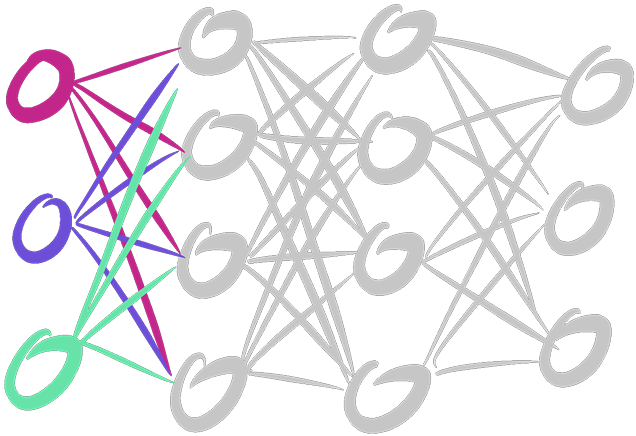
\includegraphics[width=3in]{figures/3443.png}
    \caption{A Deep MLP with 3 input nodes, 2 hidden layers with 4 nodes each, and 3 output nodes.}
    \label{3443}
\end{figure}
Lastly, the ``seed" parameter refers to creating a random seed for determining the weights, and the ``DEBUG" parameter determines whether or not the debug settings will be turned on or off. This includes various statements that print to terminal for development purposes.

After setting some initial attributes, such as the input and expected output values, the list of all weights and biases are instanced as a random value between $\pm \frac{2}{3}$. There are also two lists that are used to store the training and validation errors throughout the training process. These data are used for not only visualization, but can also be used to prevent over fitting the data. Finally, a dictionary of activation functions is stored. This is so that an activation function can be specified and called during forward or back propagation.

After the network is initialized, it needs to be trained. The second major method is the ``train" method, which runs a loop of epochs until a specified number is reached.

\lstinputlisting[firstnumber=103, firstline=103, lastline=107, caption=The ``train()" method is a loop that calls the ``calc\_err()" method repeatedly.]{src/deepmlp.py}

This method has several important keyword arguments. The ``function'' argument is a string that specifies the activation function being used in the network. The ``epochs" argument is a specified number of loops that the train method will execute. Using a fixed number of epochs is a useful constant for experimenting with the GA. There is a "learn\_rate" argument and a ``split" argument which specify the learning rate for gradient descent and the split between training and validation data respectively. Inside this loop is the ``calc\_err()" method which is where all of the mathematics are embedded.

\lstinputlisting[firstnumber=117, firstline=117, lastline=128, caption=``calc\_err()" method that forward or backward propagates recursively.]{src/deepmlp.py}

The ``forward\_prop()" and ``back\_prop()" methods are simply recursive implementations of the mathematics described in Chapter \ref{training}.
Moreover, back propagation applies the derivative to the appropriate activation function when training.
At the end of the training method are a few DEBUG methods that will print a status along with the weights matrices to the terminal after each epoch.
At the end of training the final weights and biases are displayed to the terminal.

The final two methods provide visuals for human interpretation.
The ``plot\_error()" method plots the training and validation error across all epochs from the training process.
This visual is useful for seeing how fast the network trained, and/or any complication during the training process.
There is also a ``adjacency\_matrix()" method that visualizes all weights matrices as a block matrix.
This visualization can be useful for performing a topological analysis on the trained network.

\section{Phenotype Class}
Now that the details of the Neural Networks have been covered, the next step is to look at the details of the GA classes.
Of the two main components of the GA, the phenotype class is the first and represents the lowest level.
Like the previous classes, there are three main methods that are called by the generation class that will be covered in detail: the constructor, ``init\_network()," and ``get\_fitness()."

\lstinputlisting[firstnumber=32, firstline=32, lastline=46, caption=The constructor for the phenotype class.]{src/phenotype.py}

For the constructor, the input parameters are the ``X" and ``y" arrays, again.
These data are needed to instance the Neural Networks.
It has to travel all the way down from the main script to the controller class, then to the generation class, from the generation to the phenotype class, all to be used to instance the Neural Network.
The keyword argument ``dna" is the encoding for the network's hyperparameters.
It is a bit-string that encodes the aforementioned set of hyperparameters: number of hidden nodes in each hidden layer, learning rate, and the activation function.
If an organism is instanced with the default keyword argument for ``dna," then a string of DNA will be randomly created.
This is the case when creating generation 0.
Otherwise, the ``dna" kwarg that is passed into the constructor becomes the DNA bit-string for that organism.
(This is all handled by the if statement of the ``get\_genes()" method at the end of the constructor).
Then the DNA is separated into its various smaller components and decoded into the attributes representing the hyperparameters.

Once the organism has been instanced, it is ready for the genes to instance a new Neural Network.

\lstinputlisting[firstnumber=66, firstline=66, lastline=69, caption=Method that instances a network from the genes that have been decoded from the DNA.]{src/phenotype.py}

This method is very simple because it instances a Neural Network from the deepMLP class and passes in ``X" and ``y." It then uses the genes for ``layers" and eventually the other keyword arguments for the training.

The third method is also very simple, but essential for the generation class.

\lstinputlisting[firstnumber=85, firstline=85, lastline=91, caption=Method that trains the organism's network and extracts the average fitness from the last epoch.]{src/phenotype.py}

This method calls the aforementioned ``train" method from the deepMLP class. This is when the GA trains the networks it has instanced. Then, the validation error from the final epoch becomes the fitness for that organism. The lower the error of a particular network after a fixed number of epochs is, the better that network has performed. In other words, the fitness for this GA is a minimization of this error.

\section{Generation Class}
The generation class is the object that packages the phenotypes together so the controller class can operate smoothly.
There are four important methods in this class that are called by the controller class. Once again, the first one is the constructor.

\lstinputlisting[firstnumber=43, firstline=43, lastline=51, caption=The constructor for the generation class.]{src/generation.py}

The constructor first sets the generation's ID number and then passes in the ``X" and ``y" arrays from the controller.
Afterwards, the fixed population size is set and the various fitness history arrays.
The fitness histories are lists for storing the fitness data across every generation.
This is used later for visualizing the evolution process.
After the fitness history attributes are created, the last thing the constructor does is actually build generation 0.
This is done by instancing $n$ organisms all with random DNA, where $n$ is the specified population size.

After generation 0 has been created, the controller will calculate each phenotype's fitness. The fitness values of each individual are then assessed for the reproduction phase.
This is repeated over a specified number of generations and calls two additional methods in the generation class: ``calc\_fitness()" and ``next\_generation()."

\lstinputlisting[firstnumber=68, firstline=68, lastline=76, caption=Method that has each phenotype's network train to obtain its fitness.]{src/generation.py}

The ``calc\_fitness()" method instances the Neural Networks for each organism from the organism's DNA, and then gets the fitness value for that organism.
Recall, this involves training the network and getting the validation error from the final epoch.
After this process is complete for every organism in the generation, the ``organize()" method sorts the generation list to prepare for the re-population phase.
Also nested in the ``organize()" method is the fitness re-scaling algorithm.
This re-scales the fitness scores to better distribute the organisms by fitness.
This is the same fitness scaling algorithm as presented by Dr. Goldberg \cite{Goldberg:1989:GAS:534133}.

When the ``calc\_fitness()" method has completed, the ``next\_generation" method is called next. This method calls three additional nested methods.

\lstinputlisting[firstnumber=146, firstline=146, lastline=151, caption=Method that creates the next generation of organisms and replaces the old generation.]{src/generation.py}

The elitism method picks the first two organisms from the generation.
Since the generation has been sorted by fitness, the first two are the most elite organism.
Then, they are put together to reproduce two unique organisms for the next generation. These four organisms are appended to the next generation.

Following this process, the ``repopulate()" method applies the same reproduction algorithm, but to random pairs of organisms using the roulette wheel method and the re-scaled fitness values. This process is repeated until the next generation reaches the same population as the previous generation.

The ``update\_generation()" method replaces the old generation with the new one, and accumulates the generation ID by one. At the end of each generation some data about the fitness of the generation are printed to the terminal. This whole process repeats until the specified number of generations is reached.

At the end of evolution, several different plotting methods are called to produce visuals of the results.
These visuals will be presented in Chapter \ref{results}, but below is the source code for some of the graphs that will appear.

\lstinputlisting[firstnumber=208, firstline=208, lastline=225, caption=Several methods used for plotting various results.]{src/generation.py}

The first graph, from ``plot\_total\_fitness()" is a simple graph that plots the total fitness (across every organism in the generation) over the total number of generations. The second graph, from ``plot\_fitness()" plots the three other fitness metrics that are measured each generation: best of the generation, worst of the generation, and the generation average.

\section{Controller and Main Classes}
At the top of the class totem pole we have the controller. This class' constructor is the main function that runs the entire program. This style follows closely with object oriented conventions that are taught at Binghamton University.
They allow for an overall cleaner and more organized presentation and execution of the source code; the cleaner the code, the easier it is to locate and eliminate bugs!

\lstinputlisting[firstnumber=25, firstline=25, lastline=38, caption=Contructor for the controller class. This runs the entire GA from the Neural Network training all the way to organism breeding.]{src/controller.py}

The controller passes in ``X" and ``y" data for training the Neural Networks. Additionally, the keyword arguments assign the parameters for the GA, namely the population size of each generation and the total number of generations in the whole simulation. For this project, there are two ``toy" data sets for the GA to evolve parameters for. The first one represents a simple exclusive OR (XOR) relationship which is presented in table \ref{truth1}.

\begin{table}[hbt!]
    \centering
    \caption{Truth table for exclusive or (XOR)}
    \begin{tabular}{c|c||c}
    \textbf{input} & \textbf{input} & \textbf{output}\\
    \hline
    \hline
    0 & 0 & 0\\
    0 & 1 & 1\\
    1 & 0 & 1\\
    1 & 1 & 0\\
    \end{tabular}
    \label{truth1}
\end{table}
The second data set is just a simple 4-D input replication.
Table \ref{truth2} illustrates a few examples of the input replication relationship.
\begin{table}[hbt!]
    \centering
    \caption{Truth table for 4-D input replication.}
    \begin{tabular}{c|c|c|c||c|c|c|c}
    \textbf{input} & \textbf{input} & \textbf{input} & \textbf{input} & \textbf{output} & \textbf{output} & \textbf{output} & \textbf{output}\\
    \hline
    \hline
    0 & 0 & 0 & 0 & 0 & 0 & 0 & 0\\
    0 & 1 & 1 & 0 & 0 & 1 & 1 & 0\\
    1 & 1 & 1 & 0 & 1 & 1 & 1 & 0\\
    1 & 0 & 1 & 0 & 1 & 0 & 1 & 0\\
    \end{tabular}
    \label{truth2}
\end{table}

The ``main()" method of the controller is called at the end of the constructor. This is where everything happens. Generation 0 is instanced, evolved over the specified number of generations, and the results are displayed through the figures and terminal. At the end, the best network, and its hyperparameters are printed to the terminal.

The controller class is instanced in its own main program. The main script generates the toy data and passes it into the controller along with the keyword arguments.

\lstinputlisting[firstnumber=80, firstline=80, lastline=84, language=Python, caption=Main program that instances the controller and passes in the data for training.]{src/main-xor.py}

This concludes the detailed description of the implementation of the project. Obviously there is a lot going on, but once everything is unpacked and presented in digestible pieces, the process becomes much easier to understand.

\chapter{Results from Experiments}
\label{results}
In this chapter, we will first cover the results from experiments run on the two sample data sets introduced in the previous chapter. We will first explore the results from the XOR gate data, and then  the results from the input replication data. After analyzing the results, I will discuss my reflections and interpretations of the outcomes. Finally, we will explore the limitations of this project and introduce future work that can combat these shortcomings and pave a direction for more work to be done. The parameters chosen for the genetic algorithm in both experiments are 50 organisms per generation, and 100 generations of evolution in the entire simulation.

\section{XOR Gate}
Throughout the programs' evolution phase various bits of information get printed to the terminal after each generation. Figure \ref{xorend} shows the Python terminal after the last generation has finished training its Neural  Networks. At the end of the evolution, the best performing phenotype prints its DNA, and decoded network configuration to the terminal.

\begin{figure}[hbt!]
    \centering
    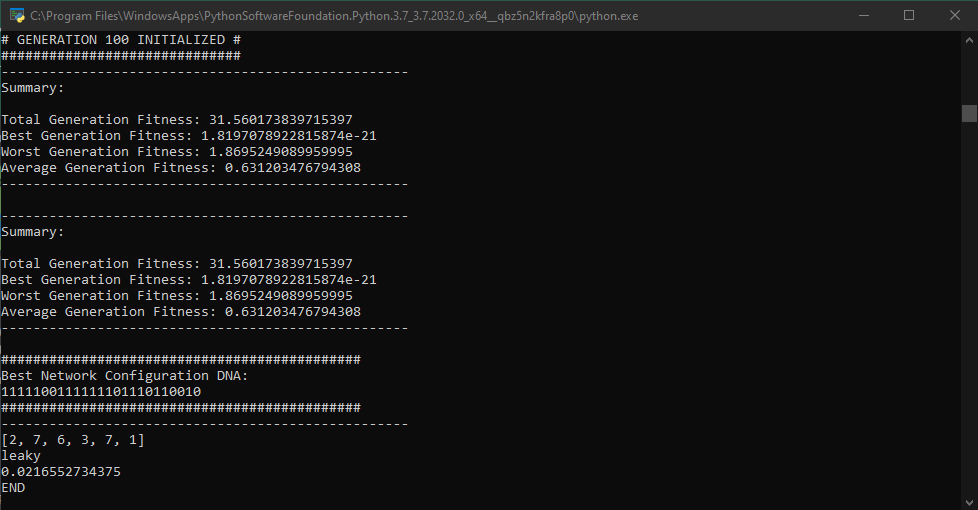
\includegraphics[width=5in]{figures/xorend.png}
    \caption{Python Terminal after the program finished evolving (XOR).}
    \label{xorend}
\end{figure}

 In this case, the DNA bit-string was ``1111100111111101110110010" which decodes to mean the layers list is [2, 7, 6, 3, 7, 1], the activation function is $\text{ReLU}_L$, and the learning rate is about 0.0217. In general, with other trials of evolving Neural Networks, similar results have been reached. That is, in all cases the best network configuration always has multiple hidden layers. We do not see the network evolving to have less hidden layers because it does not converge on a solution faster. This makes sense because XOR logic gates will not work if the network has no hidden layers, so the GA avoiding evolving less hidden layers makes sense. Another interesting property from running the evolution multiple times is that the optimal network tends to settle on ReLU type functions. The most common result was Leaky ReLU or ReLU. This result further reinforces the out performance of Sigmoid that has been historically documented.

Next, we will look at the plots produced by the program after the evolution took place.
 \begin{figure}[hbt!]
    \centering
    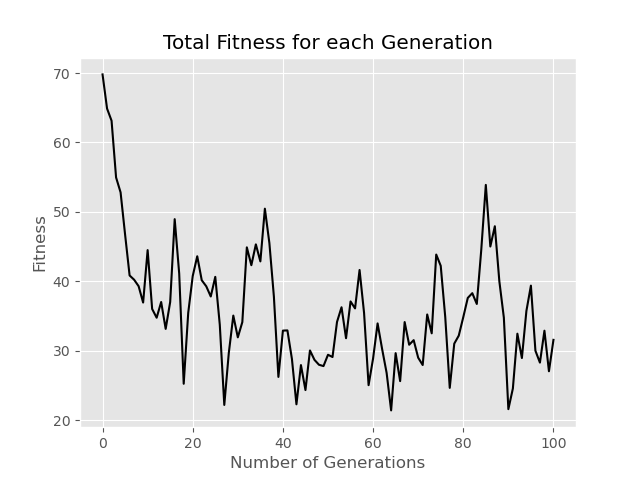
\includegraphics[width=3in]{figures/11.png}
    \caption{Plot of the sum of all fitness scores for each generation (XOR).}
    \label{xortotal}
\end{figure}
In Figure \ref{xortotal}, we see that the overall fitness reaches its best values only about twenty generations into the evolution. After this point it is likely that the best network configurations have already been discovered, and any further variances of the fitness value is due to the new organisms of the generation. Since they are new, there is no guarantee that they will be better than their parents for example.

This idea is further reinforced in Figure \ref{xorfitness}.
\begin{figure}[hbt!]
    \centering
    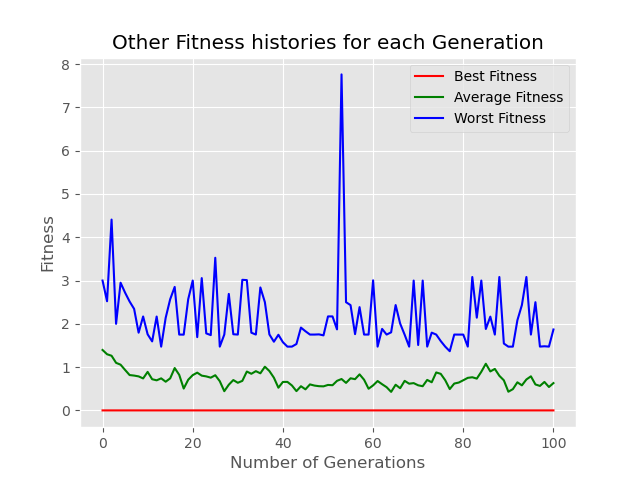
\includegraphics[width=3in]{figures/12.png}
    \caption{Plot of the best, average, and worst fitness in each generation (XOR).}
    \label{xorfitness}
\end{figure}
It appears that the near optimal network configuration is found immediately at the beginning of the evolution, since it is at this point that the best fitness score appears to remain static for the entire evolution; however, each generation is slightly optimizing the network negligible amounts each generation.

There is also a lot of variance in the worst of the generation. This is likely because of the random variations that can occur after two organisms reproduce. We see around generation 55 or so that there was some sort of mutation or ``birth defect" that cause one of the networks to perform horribly that generation. Lastly, the average fitness settles into a stable minimum state around twenty generations into the evolution akin to the total fitness graph from figure \ref{xortotal}. This makes sense because the average fitness plot is just a scaled down version of the total fitness plot.

The final plot produced by the program is Figure \ref{xorerror}: the plot of the training and validation of the best network configuration from the final generation.
\begin{figure}[hbt!]
    \centering
    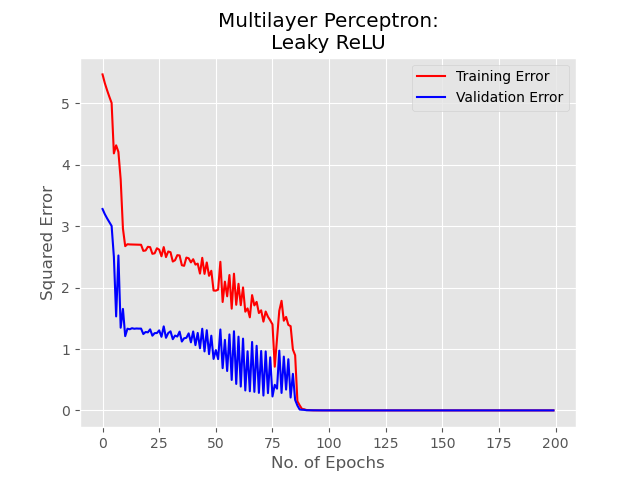
\includegraphics[width=3in]{figures/13.png}
    \caption{$\hat{E}$ value for each epoch of the best network configuration at the end of the evolution process (XOR).}
    \label{xorerror}
\end{figure}
Every network trained for 200 epochs. The shear drop off in the training error in the first couple dozen epochs is interesting. After this point the descent to its final state is more gradual. Another noteworthy structure is the series of fluctuations in the middle of the training process before finally converging on the proper weights and biases at around epoch 85.

\section{Input Replication}
Now we will look at the results from scenario 2, the input replication. While the results from scenario 1 are interesting and insightful, I believe the results from scenario 2 truly illuminate the power of Genetic Algorithms for solving these types of problems. Recall, the input replication data is trying to train the network to replicate the input as its output; reference Table \ref{truth2} as the truth table for this input.

Let's begin with Figure \ref{replicationend}, which is a terminal screenshot of the end of the evolution, with the best performing phenotype's DNA, and decoded network configuration.

\begin{figure}[hbt!]
    \centering
    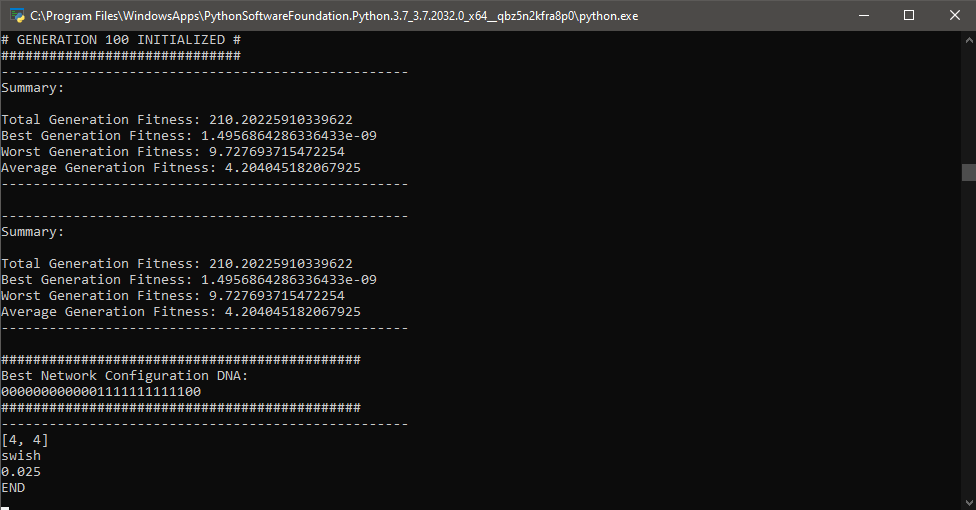
\includegraphics[width=5in]{figures/replicationend.png}
    \caption{Python Terminal after the program finished evolving (Input Replication).}
    \label{replicationend}
\end{figure}

 The resulting DNA bit-string for this example was ``0000000000001111111111100." This decodes to a simple [4, 4] layer structure, the Swish activation function $\text{Sw}$, and the learning rate is 0.025. This is a powerful result because it shows that the network evolved to have the highest possible learning rate, and the least possible number of hidden layers. This, intuitively, would be the best performing result because the network's task is so simple. If there are no hidden layers, the weights matrix will simply adjust to all be ones, and the biases will adjust to all be zeros. The genetic algorithm was able to find this solution from training a total of 5000 networks. A grid search of the same hyperparameter space is comprised of 16,777,216 network configurations, which would have taken my computer \emph{months} to run completely, instead of this roughly 1 hour runtime.

Now let's examine Figure \ref{replicationtotal}: the plot of the total fitness from every generation.
 \begin{figure}[hbt!]
    \centering
    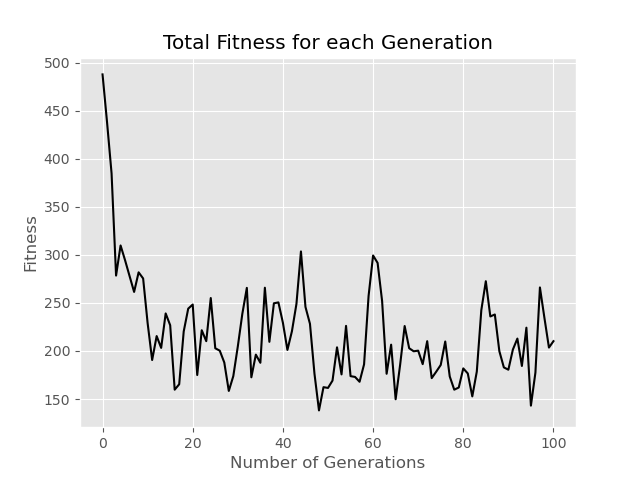
\includegraphics[width=3in]{figures/21.png}
    \caption{Plot of the sum of all fitness scores for each generation (Input Replication).}
    \label{replicationtotal}
\end{figure}
This plot is very similar to the fitness over time of the XOR data. We see it converges towards a set of near optimal solutions after about 20 epochs, and then continues searching to make minuscule improvements thereafter. Figure \ref{replicationfitness} is also very similar to the fitness plots from the XOR data. We see that near optimal solutions are found only after approximately 5 generations, however, in this plot, there seems to be many more fluctuations of the worst performing organisms in a given generation. This is most likely because the best network configuration involves no hidden layers.
If an organism mutates its hidden layer genes it could go from having no hidden layer to having 1 or two, which we would expect to not perform very well.
\begin{figure}[hbt!]
    \centering
    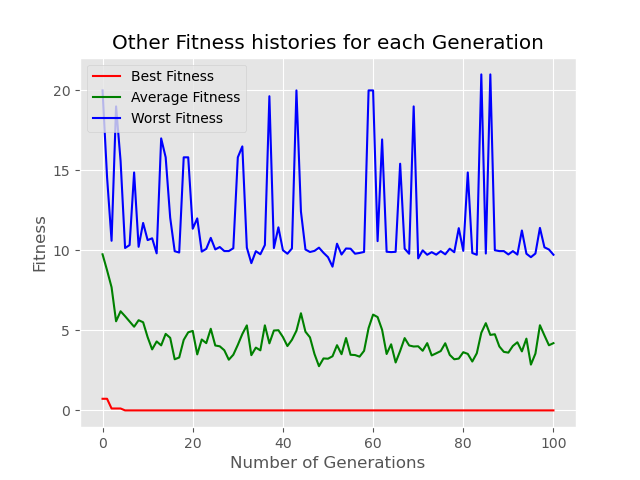
\includegraphics[width=3in]{figures/22.png}
    \caption{Plot of the best, average, and worst fitness in each generation (Input Replication).}
    \label{replicationfitness}
\end{figure}

Lastly, we will look at Figure \ref{replicationerror}.
This plot is very interesting because it shows how fast the error converges. It only takes about 25 epochs for the network to essentially be done training.
\begin{figure}[hbt!]
    \centering
    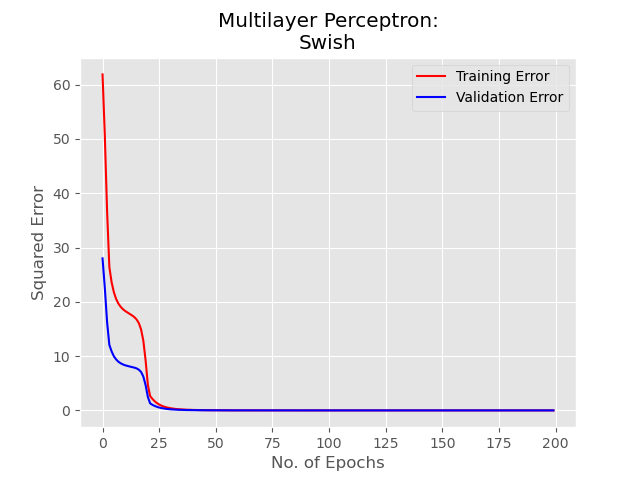
\includegraphics[width=3in]{figures/23.png}
    \caption{$\hat{E}$ value for each epoch of the best network configuration at the end of the evolution process (Input Replication).}
    \label{replicationerror}
\end{figure}
Overall, for this example I do not think the activation function is nearly as important as the network's topology, although most results end with the Sigmoid function \emph{NOT} being used. In this particular example it happened to be the Swish function, but in other runs of the evolution, ReLU, Leaky ReLU, and E-swish were all emergent results.

\section{Conclusions}
Evolutionary Algorithms are an essential component to driving machine learning progress forward. Manual search, random search, and Grid search are outdated methodologies that should be replaced by faster, and more optimal searching solutions, like evolutionary algorithms.

The input replication result shows a network that was predisposed to having several hidden layers evolve to have none. It was able to find this solution from training a total of 5000 networks, which implies it searched less than 5000 possible parameter combinations. By contrast, A grid search of the same set of hyperparameter would have to train 16,777,216 networks. Although the grid search would most likely produce a more optimal configuration, it would be more optimal only negligibly so. On larger scales, the benefits to using an evolutionary algorithms are astronomical to the efficiency and optimization to our machine learning infrastructure.

\section{Limitations and Future Work}

The most obvious next step of exploration is with data. The use of the two tow data sets for this project are perfect for discovering the capabilities of the Genetic Algorithm approach to searching for hyperparameters. However, without the validation of a data set that mimics the real world more accurately, there is no good way to emphasize the application potential in real world machine learning. It should be noted that the computational power required to execute this would also need to be greatly increased, hence why this project deals with the toy data sets.

The best way to approach this problem is to implement a well developed, stable, and consistent Neural Networks package from python such as TensorFlow. This would allow for the main focus of the project, or research, to be about exploring different large scale data sets, and different types of evolutionary algorithms. Additional features could be added to this framework such as something to signal the evolution process to stop, so a fixed number of generations is not needed to govern the process. This would save tremendously on computational effort, and thus potentially be beneficial for implementing in the everyday model training process.

\appendix
\chapter{Source Code}
All of the source code for this project can be accessed on GitHub with the following link:
\begin{center}
\bf{https://github.com/cwolosh1/hyperparameter-optimization}
\end{center}

\bibliographystyle{IEEEtran}
\addcontentsline{toc}{chapter}{References}
\bibliography{citations}


\end{document}
